% Options for packages loaded elsewhere
\PassOptionsToPackage{unicode}{hyperref}
\PassOptionsToPackage{hyphens}{url}
%
\documentclass[
  11pt,
]{article}
\usepackage{amsmath,amssymb}
\usepackage{lmodern}
\usepackage{iftex}
\ifPDFTeX
  \usepackage[T1]{fontenc}
  \usepackage[utf8]{inputenc}
  \usepackage{textcomp} % provide euro and other symbols
\else % if luatex or xetex
  \usepackage{unicode-math}
  \defaultfontfeatures{Scale=MatchLowercase}
  \defaultfontfeatures[\rmfamily]{Ligatures=TeX,Scale=1}
\fi
% Use upquote if available, for straight quotes in verbatim environments
\IfFileExists{upquote.sty}{\usepackage{upquote}}{}
\IfFileExists{microtype.sty}{% use microtype if available
  \usepackage[]{microtype}
  \UseMicrotypeSet[protrusion]{basicmath} % disable protrusion for tt fonts
}{}
\makeatletter
\@ifundefined{KOMAClassName}{% if non-KOMA class
  \IfFileExists{parskip.sty}{%
    \usepackage{parskip}
  }{% else
    \setlength{\parindent}{0pt}
    \setlength{\parskip}{6pt plus 2pt minus 1pt}}
}{% if KOMA class
  \KOMAoptions{parskip=half}}
\makeatother
\usepackage{xcolor}
\usepackage[margin=1in]{geometry}
\usepackage{graphicx}
\makeatletter
\def\maxwidth{\ifdim\Gin@nat@width>\linewidth\linewidth\else\Gin@nat@width\fi}
\def\maxheight{\ifdim\Gin@nat@height>\textheight\textheight\else\Gin@nat@height\fi}
\makeatother
% Scale images if necessary, so that they will not overflow the page
% margins by default, and it is still possible to overwrite the defaults
% using explicit options in \includegraphics[width, height, ...]{}
\setkeys{Gin}{width=\maxwidth,height=\maxheight,keepaspectratio}
% Set default figure placement to htbp
\makeatletter
\def\fps@figure{htbp}
\makeatother
\setlength{\emergencystretch}{3em} % prevent overfull lines
\providecommand{\tightlist}{%
  \setlength{\itemsep}{0pt}\setlength{\parskip}{0pt}}
\setcounter{secnumdepth}{-\maxdimen} % remove section numbering
\newlength{\cslhangindent}
\setlength{\cslhangindent}{1.5em}
\newlength{\csllabelwidth}
\setlength{\csllabelwidth}{3em}
\newlength{\cslentryspacingunit} % times entry-spacing
\setlength{\cslentryspacingunit}{\parskip}
\newenvironment{CSLReferences}[2] % #1 hanging-ident, #2 entry spacing
 {% don't indent paragraphs
  \setlength{\parindent}{0pt}
  % turn on hanging indent if param 1 is 1
  \ifodd #1
  \let\oldpar\par
  \def\par{\hangindent=\cslhangindent\oldpar}
  \fi
  % set entry spacing
  \setlength{\parskip}{#2\cslentryspacingunit}
 }%
 {}
\usepackage{calc}
\newcommand{\CSLBlock}[1]{#1\hfill\break}
\newcommand{\CSLLeftMargin}[1]{\parbox[t]{\csllabelwidth}{#1}}
\newcommand{\CSLRightInline}[1]{\parbox[t]{\linewidth - \csllabelwidth}{#1}\break}
\newcommand{\CSLIndent}[1]{\hspace{\cslhangindent}#1}
\usepackage{setspace}\doublespacing
\usepackage{lineno}\linenumbers
\usepackage[utf8]{inputenc}
\usepackage[T1]{fontenc}
\usepackage{biblatex}
\usepackage{booktabs}
\usepackage{longtable}
\usepackage{array}
\usepackage{multirow}
\usepackage{wrapfig}
\usepackage{float}
\usepackage{colortbl}
\usepackage{pdflscape}
\usepackage{tabu}
\usepackage{threeparttable}
\usepackage{threeparttablex}
\usepackage[normalem]{ulem}
\usepackage{makecell}
\usepackage{xcolor}
\ifLuaTeX
  \usepackage{selnolig}  % disable illegal ligatures
\fi
\IfFileExists{bookmark.sty}{\usepackage{bookmark}}{\usepackage{hyperref}}
\IfFileExists{xurl.sty}{\usepackage{xurl}}{} % add URL line breaks if available
\urlstyle{same} % disable monospaced font for URLs
\hypersetup{
  pdftitle={Evolution along allometric lines of least resistance: Morphological differentiation in Pristurus geckos},
  hidelinks,
  pdfcreator={LaTeX via pandoc}}

\title{Evolution along allometric lines of least resistance:
Morphological differentiation in \emph{Pristurus} geckos}
\author{}
\date{\vspace{-2.5em}}

\begin{document}
\maketitle

\begin{center}
\textbf{H{\'{e}}ctor Tejero-Cicu{\'{e}}ndez$^{1,2,*}$,  Iris Men{\'{e}}ndez$^{3}$, Adri{\'{a}}n Talavera$^{2}$, Gabriel Riaño$^{2}$, Bernat Burriel-Carranza$^{2}$, Marc Sim{\'{o}}-Riudalbas$^{2}$, Salvador Carranza$^{2}$, and Dean C. Adams$^{4}$}
\end{center}

\begin{center}17 April, 2023\end{center}

\(^{1}\)Evolution and Conservation Biology research Group, Department of
Biodiversity, Ecology and Evolution. Faculty of Biology. Universidad
Complutense de Madrid, 28040, Madrid, Spain

\(^{2}\)Institute of Evolutionary Biology (CSIC-Universitat Pompeu
Fabra), Passeig Marítim de la Barceloneta 37-49, Barcelona 08003, Spain

\(^{3}\)Museum für Naturkunde, Leibniz Institute for Evolution and
Biodiversity Science, Berlin, Germany

\(^{4}\)Department of Ecology, Evolution, and Organismal Biology, Iowa
State University, Ames, Iowa, 50010 USA

\(^{*}\)Correspondence: Héctor Tejero-Cicuéndez
\href{mailto:cicuendez93@gmail.com}{\nolinkurl{cicuendez93@gmail.com}}

\newpage

\hypertarget{abstract}{%
\section{Abstract}\label{abstract}}

Species living in distinct habitats often experience unique ecological
selective pressures, which can drive phenotypic divergence. However, how
ecophenotypic patterns are affected by allometric trends and trait
integration levels is less well understood. Here we evaluate the role of
allometry in shaping body size and body form diversity in
\emph{Pristurus} geckos utilizing differing habitats. We found that
patterns of allometry and integration in body form were distinct in
species with different habitat preferences, with ground-dwelling
\emph{Pristurus} displaying the most divergent allometric trend and high
levels of integration. There was also strong concordance between static
allometry across individuals and evolutionary allometry among species,
revealing that differences in body form among individuals were
predictive of evolutionary changes across the phylogeny at
macroevolutionary scales. This suggested that phenotypic evolution
occurred along allometric lines of least resistance, with allometric
trajectories imposing a strong influence on the magnitude and direction
of size and shape changes across the phylogeny. When viewed in
phylomorphospace, the largest rock-dwelling species were most similar to
the smallest ground-dwelling species, and vice versa. Thus, in
\emph{Pristurus}, phenotypic evolution along the differing habitat-based
allometric trajectories resulted in similar body forms at differing body
sizes in distinct ecological habitats.

\newpage

\hypertarget{introduction}{%
\section{1. Introduction}\label{introduction}}

Understanding how phenotypic diversity evolves, and elucidating the
forces that generate and maintain this diversity, are major goals in
evolutionary biology. Because adaptive evolution is the product of
natural selection, changes in ecological selection pressures are
expected to affect the evolutionary trajectory of phenotypic traits that
facilitate an organism's survival and reproduction in their habitat. The
theory of natural selection predicts that differing habitats will exert
unique ecological selection pressures on organisms, resulting in
associations between ecological and phenotypic traits. Indeed, species
inhabiting differing habitats often display functional, behavioral, or
phenotypic differences, that have presumably been the result of adaptive
diversification in their respective ecological contexts (Collar et al.
2010; Kaliontzopoulou et al. 2015; Price et al. 2015; Martinez et al.
2021; Kolmann et al. 2022). \hfill\break

One possible evolutionary outcome of ecological specialization is that
organisms inhabiting similar environments display common phenotypic
characteristics. When such patterns occur repeatedly (Losos 1992;
Schluter and McPhail 1992), this convergent evolution is treated as
strong evidence of adaptation. Indeed the ecomorphological paradigm
(Arnold 1983) is predicated, in part, on such cases, which emphasize the
strong association between the phenotypic traits that organisms display
(morphological, behavioral, or physiological) and the ecological
characteristics of their habitat that mediate organismal performance. In
vertebrates, ecomorphological trends have been well studied in numerous
taxonomic groups, and include the emblematic `ecomorphs' of Caribbean
\emph{Anolis} lizards that exploit different microhabitats (Losos 1992,
2009; Mahler et al. 2013), differential beak morphology in species of
Darwin's finches (Schluter and Grant 1984; Grant and Grant 2006; Reaney
et al. 2020), the recurring phenotypes of African lake cichlids across
ecological regimes (Albertson and Kocher 2001; Urban et al. 2022), and
the distinct body forms of freshwater fishes in benthic and limnetic
habitats (Jastrebski and Robinson 2004; Berner et al. 2008; Stuart et
al. 2017), among others. \hfill\break

While the patterns of morphological differences in distinct ecological
contexts have been well documented, less-well understood is how
ecomorphological differentiation has been influenced by trait
covariation associated with body size differences (i.e., allometry). The
study of size-related changes in anatomical traits has a long history in
evolutionary biology (Huxley 1932; Jolicoeur 1963; Gould 1966;
Klingenberg 1996; Zelditch and Swiderski 2022). One reason for this is
that nearly all traits covary strongly with overall body size (Jolicoeur
1963; Gould 1966; Bookstein 2022), and as such, the effects of allometry
on patterns of phenotypic diversity are expected to be considerable.
Further, allometric patterns manifest widely across differing levels of
biological organization: from variation across individuals at differing
stages or ages (i.e., ontogenetic allometry), to variation across
individuals in a single ontogenetic stage within a population or species
(i.e., static allometry), to variation across species of differing
sizes, as described by evolutionary allometry (see Cock 1966;
Klingenberg and Zimmermann 1992). Indeed, across vertebrates, numerous
studies have shown that a sizeable proportion of overall phenotypic
variation is related to interspecific differences in body size (Pyron
and Burbrink 2009; Piras et al. 2010; Cardini and Polly 2013; e.g.,
Sherratt et al. 2014; Cardini et al. 2015; Bright et al. 2016; Bardua et
al. 2021; Felice et al. 2021; Zelditch and Swiderski 2022). When viewed
from this perspective, patterns of ontogenetic and evolutionary
allometry are thought to play a decisive role in shaping patterns of
phenotypic diversification across the tree of life. \hfill\break

However, allometry can also act as a restraining force on evolution by
limiting the breadth of phenotypes that can be realized (Bright et al.
2019). This occurs because trait correlations influence the degree to
which phenotypic variation is exposed to selection (Wagner and Altenberg
1996). Thus, the integration among traits can constrain phenotypic
change in certain directions, or enhance variation along other
phenotypic axes (Schluter 1996; Wagner and Altenberg 1996; Wagner and
Zhang 2011; Klingenberg and Marugán-Lobón 2013; Goswami et al. 2014,
2016; Felice et al. 2018; Navalón et al. 2020). Further, because nearly
all linear traits covary strongly with overall body size, allometric
trends could be considered the quintessential expression of phenotypic
integration (Zelditch and Swiderski 2022; Bookstein 2022). Thus, when
evaluating ecophenotypic differences among taxa, it is important to
consider how allometric trends of trait covariation influence such
patterns (e.g., Esquerré et al. 2017; Patterson et al. 2022; Chatterji
et al. 2022). \hfill\break

The Afro-Arabian geckos in the genus \emph{Pristurus} afford the
opportunity to elucidate the interdigitating effects of allometry and
habitat specialization on clade-level patterns of phenotypic diversity.
From an evolutionary perspective, \emph{Pristurus} geckos are an ideal
system to investigate the role of different factors in evolutionary
history. They are found in both insular and continental settings, which
are known to impose differential ecological selection pressures
resulting in distinct evolutionary trajectories of species and clades
(Losos and Ricklefs 2009). They are also distributed in the contact zone
between Africa and Eurasia, a region of high biogeographic interest
which has been the epicenter of major faunal interchanges and complex
geologic and environmental processes (Kappelman et al. 2003;
Tejero-Cicuéndez et al. 2022). The study of evolutionary dynamics in
\emph{Pristurus} and other Afro-Arabian taxa is also important
biologically, as our understanding of the dynamics of biological systems
in remote arid regions is generally neglected and understudied (Durant
et al. 2012). Furthermore, prior work on this system (Tejero-Cicuéndez
et al. 2021a) has revealed that the colonization of ground habitats has
been a trigger of morphological change, specifically reflected in an
increase in body size and shape disparity. Interestingly, some
ground-dwelling species are among the largest of the genus and also show
increased relative head sizes and limb proportions, while some other
species with this ecological specialization have evolved to be among the
smallest of the group. Additionally, among the species exploiting rocky
habitats (the most common ecological feature in \emph{Pristurus}), there
are also species with both considerably large and small body sizes
(Tejero-Cicuéndez et al. 2021a). What remains unexplored, however, is
how the evolution of body form is related to differences in body size
and whether habitat specialization has an impact in this shape-size
relationship. \hfill\break

In this study, we employed a combination of multivariate morphometric
and phylogenetic comparative analyses to interrogate macroevolutionary
patterns of evolutionary allometry in \emph{Pristurus} geckos of
Afro-Arabia. Using phenotypic, phylogenetic, and ecological data, we
first characterized allometric trends in body form in the group, to
discern the extent to which evolutionary allometric trends across the
phylogeny aligned with habitat-based static allometry for species
occupying distinct ecological regimes. We then examined changes in
allometric trends across the phylogeny, and linked these patterns to
overall phenotypic integration, diversification in morphospace, and
habitat utilization among taxa. Our analyses reveal that patterns of
evolutionary allometry across species align with allometric trends among
individuals, and that differing habitat-based allometric trajectories
have resulted in similar body forms at differing body sizes in distinct
ecological regimes. Thus, patterns of phenotypic diversification in
\emph{Pristurus} are the outcome of an interplay between ecological
specialization and size-form changes evolving along habitat-specific
allometric trajectories in the group.

\hypertarget{materials-and-methods}{%
\section{2. Materials and Methods}\label{materials-and-methods}}

\hypertarget{a-data}{%
\subsection{(a) Data}\label{a-data}}

We used a combination of phenotypic, phylogenetic, and ecological data
to characterize and evaluate intra- and interspecific allometric trends
in \emph{Pristurus}. The data utilized here were obtained from our prior
work on this system (Tejero-Cicuéndez et al. 2021a, 2022), and are
briefly described here. First we used a time-calibrated molecular
phylogeny of squamates that included all members of the genus
\emph{Pristurus}, including several currently undescribed taxa. The tree
was estimated in a Bayesian framework, using five mitochondrial markers,
six nuclear markers, and 21 calibration points (Tejero-Cicuéndez et al.
2022). Next we categorized each species as belonging to one of three
ecological habitat groups (ground-dwelling, rock-dwelling, or
tree-arboreal). Habitat designations were based on substrate preferences
and habitat use as found through extensive field observations described
in the primary literature (Arnold 1993; Arnold 2009, and references
therein). Finally, we obtained a phenotypic data set containing body
size (snout-vent length: SVL) and eight linear measurements (Figure 1)
that described overall body form: trunk length (TL), head length (HL),
head width (HW), head height (HH), humerus length (Lhu), ulna length
(Lun), femur length (Lfe), and tibia length (Ltb) (Tejero-Cicuéndez et
al. 2021a). We restricted our study to those species represented by nine
or more individuals; resulting in a dataset of 687 individuals from 25
species (invidivuals per species: mean=27; min = 9, max = 56). All
specimens used in this study were adults, and thus patterns of
ontogenetic allometry could not be explored. Species in the phenotypic
dataset were then matched to the phylogeny, which was subsequently
pruned to the final topology. All measurements were log-transformed
prior to statistical analyses. Additional details regarding data
collection and formal descriptions of each linear measurement may be
found in the original sources (Tejero-Cicuéndez et al. 2021a, 2022). The
data are available on DRYAD:
\url{https://doi.org/10.5061/dryad.xwdbrv1f6} (Tejero-Cicuéndez et al.
2021b).

\hypertarget{b-statistical-and-comparative-analyses}{%
\subsection{(b) Statistical and Comparative
Analyses}\label{b-statistical-and-comparative-analyses}}

We conducted a series of analyses to interrogate allometric trends,
patterns of integration, and macroevolutionary changes in allometry,
relative to differentiation in body form. First we characterized
evolutionary allometry in the genus by performing a phylogenetic
multivariate regression of body form on body size (i.e., SVL), using the
species means as data. We then evaluated patterns of static allometry
among individuals using a pooled within-species regression (sensu
Klingenberg 2016). Here a pooled within-species dataset was generated by
obtaining residuals for all individuals relative to their respective
species means, which were then pooled across species. This dataset was
then used in a multivariate regression to obtain an overall estimate of
static allometry among individuals. By first removing species-specific
differences, this procedure partials out trends of evolutionary
allometry from the data, enabling patterns of static and evolutionary
allometry to be disentangled. From both the species-level and the
individual-level analyses, we obtained the set of regression
coefficients, which respectively described the trajectories of
evolutionary and static allometry in morphospace. We then calculated the
difference in their direction in morphospace to discern the extent to
which patterns of static allometry at the individual level were
concordant with evolutionary allometric trends across species.
\hfill\break

Next we used the pooled within-species dataset to determine whether
trends in static allometry differed across habitat groups. This was
accomplished by performing a multivariate analysis of covariance, with
body size (\(SVL\)), \(habitat\), and \(SVL \times habitat\) as model
effects. Significance of model effects was evaluated using 999
iterations of a permutation procedure, where residuals from a reduced
model were randomly permuted in each permutation (RRPP), model
statistics were recalculated, and used to generate empirical null
sampling distributions to evaluate the observed test statistics
(following Freedman and Lane 1983; Collyer and Adams 2007; Collyer et
al. 2015). In this analysis, no variation was attributable to the
\(habitat\) effect, as the pooled-within species data are mean-centered
for both the dependent and independent variables. However, any
differences in multivariate allometric slopes among habitats will be
discernable, and revealed by a significant \(SVL \times habitat\)
interaction. To evaluate this possibility, we compared the direction of
multivariate allometric vectors for each habitat group to one another,
and to a vector representing multivariate isometry, by calculating
pairwise angular differences in their direction in morphospace, and
evaluating these relative to empirical sampling distributions obtained
through RRPP (Collyer and Adams 2007; Adams and Collyer 2009; Collyer
and Adams 2013). Here, residuals were obtained from a common isometry
reduced model, whose common slope component described a pattern of
multivariate isometry, and whose intercepts allowed for differences in
least-squares means among groups. Patterns of multivariate allometry
relative to body size were visualized via regression scores (Drake and
Klingenberg 2008) and predicted lines (Adams and Nistri 2010), based on
the coefficients and fitted values from the linear model described
above. \hfill\break

Additionally, because allometry describes the extent to which traits
covary with body size and with each other (i.e., integration), we
conducted an analysis of integration. Here we characterized the extent
of morphological integration in body form for individuals within each
habitat group using the pooled within-species dataset, and by
summarizing the dispersion of eigenvalues of their respective trait
covariance matrix (Pavlicev et al. 2009). This measure (\(V_{rel}\)) was
subsequently converted to an effect size (a \(Z\)-score), which
quantified the strength of morphological integration (Conaway and Adams
2022). We then performed a series of two-sample tests to compare the
strength of morphological integration across habitat groups, following
the procedures of Conaway and Adams (2022). Additionally and for
comparison, we repeated these analyses on the set of size-standardized
trait data, found as a set of shape ratios (Mosimann 1970) where each
trait was divided by body size (Supplementary Material). \hfill\break

To determine the extent to which static and evolutionary allometry were
concordant, we evaluated the directions in morphospace of both the
evolutionary (species-level) and static (habitat-based) allometric
trends. Specifically, we obtained the set of regression coefficients
from both the phylogenetic multivariate regression and the multivariate
analysis of covariance analyses above, and calculated the angular
difference in direction between the evolutionary allometry trajectory
and the static allometry trend for each habitat group. The observed
angles were then statistically evaluated relative to empirical sampling
distributions obtained through permutation (RRPP), based on the common
isometry model described above. \hfill\break

Next, to discern how allometric trends resulted in the evolution of
distinct body forms, we examined changes in relative body form across
the phylogeny. Here we treated the head dimensions and limb dimensions
separately, as allometric trends could potentially differ between these
body regions due to differential functional or selective constraints
(Kaliontzopoulou et al. 2010). Because both the head and limb data were
multivariate, we used regression scores (sensu Drake and Klingenberg
2008) of a multivariate regression of head traits versus SVL and limb
traits versus SVL to represent the allometric trends in each dataset. We
then measured the mean residuals of each species to the inferred
allometric trend, which described the extent to which head and limb
proportions of species were greater or smaller than expected for their
body size. The species residuals were then mapped on the phylogeny of
\emph{Pristurus} using a Brownian motion model of evolution, to
qualitatively evaluate shifts in head and limbs proportionality across
the phylogeny for the group. Similarly, within-species patterns of
static allometry were visualized by plotting regression scores versus
SVL for both head and limb traits separately. \hfill\break

Finally, to relate within-species allometric trends with patterns of
phenotypic diversification in the group we generated a phylomorphospace
(sensu Sidlauskas 2008), based on a principal component analyses (PCA)
of the size-standardized species means (i.e., relative body proportions)
obtained from a phylogenetic regression (see Tejero-Cicuéndez et al.
2021a). Here, phenotypic similarities among species, relative to their
phylogenetic relationships and habitat affiliations, were observed. A
similar phylomorphospace was constructed for species means not corrected
for body size, and the phenotypic disparity among species means in each
habitat was calculated and subsequently compared (Supplementary
Material). Additionally, anatomical changes associated with allometric
trends across taxa were visually depicted via representative specimens
from the largest and smallest ground-dwelling species (scaled to unit
size), and specimens from a large and small rock-dwelling species, to
aid in describing these allometric trends. All analyses were conducted
in R 4.2.1 (R Core Team 2022), using \texttt{RRPP} version 1.3.2
(Collyer and Adams 2018; Collyer and Adams 2022) and \texttt{geomorph}
4.0.5 (Baken et al. 2021a) for statistical analyses and the
\texttt{tidyverse} version 1.3.0 (Wickham et al. 2019),
\texttt{phytools} version 0.7-77 (Revell 2012), and a modified version
of the function \texttt{ggphylomorpho}
{[}\url{https://github.com/wabarr/ggphylomorpho}{]} for data
manipulation and visualization, as well as scripts written by the
authors (Supplementary Material).

\hypertarget{results}{%
\section{3. Results}\label{results}}

Using phylogenetic regression, we found significant evolutionary
allometry in body form across species (\(N_{sp}=25\); \(F = 217.9\);
\(Z =5.53\); \(P < 0.001\)). Likewise, when static allometry in body
form was examined across individuals, a similar pattern was observed
(\(N_{ind}=687\); \(F = 1176.9\); \(Z =8.24\); \(P < 0.001\)). Further,
the vectors of regression coefficients between the two analyses were
oriented in a similar direction and were nearly parallel in morphospace
(\(\theta = 5.64^\circ\)). This revealed that the pattern of
multivariate allometry across individuals was largely concordant with
macroevolutionary trends of interspecific static allometry among species
of \emph{Pristurus} across the phylogeny. \hfill\break

Our analyses also exposed significant differences in the allometry of
body form among \emph{Pristurus} utilizing distinct habitats (Table 1).
Further, pairwise comparisons of multivariate allometric vectors
revealed that patterns of static allometry in each habitat differed
significantly from isometry, indicating the presence of multivariate
allometry in each (Table 2). Additionally, comparisons identified that
ground-dwelling \emph{Pristurus} displayed the most distinct allometric
trend as compared with \emph{Pristurus} occupying both the rock and tree
habitats (Table 2; Figure 2). Here, regression coefficients of each
trait versus size (Supplementary Material) revealed that ground-dwelling
\emph{Pristurus} exhibited higher coefficents for head traits as
compared with rock-dwelling and tree-dwelling taxa
(\(\beta_{ground}>\beta_{rock}\);\(\beta_{ground}>\beta_{tree}\)). By
contrast, coefficients for limb traits were somewhat smaller for
ground-dwelling \emph{Pristurus} as compared with other taxa
(\(\beta_{ground}<\beta_{rock}\);\(\beta_{ground}<\beta_{tree}\)). Thus,
these findings implied that within species, larger individuals of
ground-dwelling \emph{Pristurus} displayed proportionately larger heads
and slightly smaller limbs as compared with large individuals in taxa
utilizing other habitat types. Visualizations of the allometric trends
(Figure 2) confirmed these statistical findings, and indicated that the
allometric trajectory in ground-dwelling \emph{Pristurus} was more
extreme as compared with either rock- or tree-dwelling \emph{Pristurus}.
\hfill\break

Examination of patterns of trait covariation for the pooled
within-species data revealed strong levels of morphological integration
in the ground and tree ecotypes, with lower levels of integration
displayed in the rock habitat. Subsequent two-sample tests revealed that
the strength of morphological integration was significantly greater in
both ground-dwelling and tree-dwelling \emph{Pristurus} than in those
utilizing rock (\(Z_{ground-rock}=6.05\); \(P << 0.001\);
\(Z_{tree-rock}=4.07\); \(P << 0.001\)). Levels of morphological
integration did not differ between ground and tree-dwelling
\emph{Pristurus} (\(Z_{tree-rock}=0.38\); \(P = 0.702\)). Finally, when
body size was taken into account, levels of integration dropped
considerably, though the overall pattern and differences among habitat
groups remained the same (Supplementary Material). \hfill\break

Comparisons of evolutionary allometry with static allometry in each
habitat revealed substantial concordance between allometric trends
across these levels. Here, vectors of regression coefficients
representing static allometry within habitat groups were oriented in
very similar directions with the regression vector representing
evolutionary allometry, with small pairwise angles between them
(\(\theta: 5.8^\circ\rightarrow7.2^\circ\)). Subsequent permutation
tests indicated no differences in direction between the regression
vector representing evolutionary allometry and the static allometry
vectors for \emph{Pristurus} in both the ground or tree habitats,
indicating strong congruence between them (Table 3). By contrast,
rock-dwelling \emph{Pristurus} differed most in their static allometry
trend relative to patterns of evolutionary allometry. Notably, static
allometry in ground-dwelling \emph{Pristurus} was most similar to trends
of evolutionary allometry, displaying the smallest angular difference in
direction when compared to evolutionary allometry. Overall, these
findings implied that phenotypic evolution across species aligned
closely with directions of allometric variation within habitat groups at
the individual level, describing a trend where larger individuals -- and
larger ground-dwelling species -- exhibited disproportionately larger
heads and limbs, while smaller individuals -- and smaller
ground-dwelling species -- displayed disproportionately smaller heads
and limbs. \hfill\break

Mapping the residuals of phylogenetic regression onto the phylogeny
showed that large ground-dwelling species displayed greater head
proportions than large rock-dwelling species, who exhibited smaller
heads relative to body size (Figure 3A). Conversely, the opposite
pattern was observed when comparing small species utilizing these
habitats: ground-dwelling species showed small relative head proportions
while rock-dwelling species displayed generally larger head proportions.
In contrast, limb shape showed more variable patterns. Although all
large ground-dwelling species consistently displayed large relative limb
proportions, large rock-dwelling species were more variable in this
trait, with \emph{P. insignis} exhibiting large and \emph{P.
insignoides} small limb proportions. For small species, shifts in
relative limb proportions seemed more independent of habitat
utilization, since there were differences in limb residuals both within
rock- and ground-dwelling species (Figure 3B). Likeweise, static
allometry trends within species revealed that ground-dwelling species
generally displayed steeper allometric patterns in head proportions as
compared with rock-dwelling species (Figure 4). Overall there was
general concordance across taxa in terms of trends of multivariate
allometry, affirming that the association between evolutionary allometry
and habitat-based static allometry was robust. \hfill\break

Viewing differentiation in relative body proportions in \emph{Pristurus}
in phylomorphospace (Figure 5) revealed broad overlap among habitat
groups in the first few dimensions, though arboreal (tree-dwelling)
species were somewhat more constrained in morphospace. Rock-dwelling
species occupied a slightly larger region of morphospace as compared
with the other groups, though this pattern was not statistically
significant (Supplementary Material). Intriguingly, when viewed in
relation to body size, large \emph{Pristurus} species were not localized
to a particular region of morphospace, nor were smaller species.
Instead, the largest rock-dwelling species were found in close proximity
to the smallest ground-dwelling species, indicating that they were
similar in relative body proportions. Likewise, the smallest
rock-dwelling species were found close to large ground-dwelling species
in morphospace, indicating they displayed similar body proportions as
well. \hfill\break

Finally, when representative specimens were scaled to a similar body
size (Figure 6), the anatomical consequences of differences in
allometric trends on body form became apparent. Here, larger
ground-dwelling \emph{Pristurus} species displayed disproportionately
larger heads and limbs as compared with large \emph{Pristurus} species
utilizing other habitat types. Conversely, smaller rock-dwelling species
were found to have disproportionately larger heads and limbs as compared
with smaller ground-dwelling species. These patterns corresponded
closely with those identified in morphospace (Figure 5), where large
ground-dwelling species were similar in body form to small rock-dwelling
species, while small ground-dwelling species were similar in body form
to large rock-dwelling species (Figure 6). Thus, synthesizing the
patterns revealed in the phylomorphospace with those from the other
analyses revealed that the same body proportions could be obtained in
different ways, as determined by subtle differences in allometric slope
across habitats, combined with body size differences. As such, species
with similar body proportinos displayed differing overall size, were
found in distinct habitats, and exhibited different allometric trends.
\hfill\break

\hypertarget{discussion}{%
\section{4. Discussion}\label{discussion}}

Elucidating the selective forces that generate patterns of phenotypic
diversity is a major goal in evolutionary biology. For species that
utilize distinct habitats, disentangling the causes of phenotypic
differentiation across those habitats is essential for our understanding
of how natural selection operates and how evolution proceeds. In this
study, we evaluated the role of potential drivers of body form
differentiation in the geckos of the genus \emph{Pristurus}. To this
end, we compared allometric trends and levels of integration among
\emph{Pristurus} occupying distinct habitats, interrogated allometric
patterns at both the static and evolutionary levels, and related these
trends to diversification in body form. Our findings have several
important implications for how ecological specialization, phenotypic
integration, and body form evolution along allometric trajectories
relate to patterns of phenotypic diversity generally, and the evolution
of phenotypic diversification in \emph{Pristurus} in particular.
\hfill\break

First, our analyses revealed that patterns of allometry in body form and
morphological integration are relatively distinct in ground-dwelling
\emph{Pristurus} lizards, as compared with \emph{Pristurus} occupying
other habitats. Specifically, we found that multivariate vectors of
regression coefficients differed significantly from what was expected
under isometry (Table 2) for taxa utilizing all habitat types (ground,
rock, tree), indicating that in \emph{Pristurus}, allometric scaling
patterns predominate. Further, our interrogation of allometric trends
revealed differences between habitat types, where ground-dwelling
\emph{Pristurus} displayed steeper allometric trends for head traits as
compared with rock and tree-dwelling taxa. Biologically, these patterns
revealed that not only does shape differ between large and small
\emph{Pristurus}, but this pattern differs across habitat types.
Specifically, large ground-dwelling \emph{Pristurus} present
disproportionately larger heads relative to large individuals in other
habitats, while small ground-dwelling \emph{Pristurus} exhibit
disproportionately smaller heads (Figure 3). These findings are
consistent with previous work at the macroevolutionary level
(Tejero-Cicuéndez et al. 2021a), where large ground species were also
found to display disproportionately large heads. \hfill\break

Second, our findings revealed that within species, rock-dwelling
\emph{Pristurus} show a converse pattern, where smaller individuals
displayed relatively larger heads, while larger individuals have smaller
heads relative to their body size. These allometric patterns also
corresponded with findings at macroevolutionary scales (Tejero-Cicuéndez
et al. 2021a), where similar patterns at the species level were
observed. Regarding relative limb proportions, we found a high
variability among small rock-dwelling species rather than a common
pattern (Figure 3B). Indeed, earlier work in the subclade comprising
several of these species (the \emph{P. rupestris} species complex) found
two well-differentiated phenotypes in populations of these lineages
segregated by elevation (Garcia-Porta et al. 2017). These two ecotypes,
defined as `slender' and `robust', differed in their head and limb
characteristics. Our work is consistent with this, and extends these
patterns to the allometric realm. Tejero-Cicuéndez et al. (2021a) also
performed habitat ancestral estimation, finding that the rock habitat
was the most likely ancestral condition in the group, with subsequent
colonization by \emph{Pristurus} of ground habitats. When patterns of
allometry are viewed through this lens, it suggests the hypothesis that
habitat shifts from rock-dwelling to ground-dwelling incurred a
concomitant evolutionary shift in allometric trajectories as well (Adams
and Nistri 2010). Indeed, our analyses are consistent with this
hypothesis, as allometric trends are inferred to be more rock-like
towards the root of the \emph{Pristurus} phylogeny (Figure 3), with
subsequent shifts along branches leading to ground-dwelling species.
This further suggests that the segregation in body size and shape
through differential allometric relationships across habitats responds
to adaptive dynamics concerning the colonization of new habitats. Thus,
in \emph{Pristurus}, there is support for the hypothesis that
colonization of ground habitats has been a trigger for morphological
change (Tejero-Cicuéndez et al. 2021a), as there appears to be a link
between shifts in allometric trajectories as a result of habitat-induced
selection, and differential patterns of body form observed across taxa.
Similar patterns have been observed in other taxa, where differences in
allometric trajectories are associated with ecological differences
across species (Esquerré et al. 2017; Patterson et al. 2022; Chatterji
et al. 2022). More broadly, these findings are consistent with prior
discoveries in other lizards, where the differential selective pressures
imposed by rocky and ground habitats have resulted in the
differentiation of head and limb morphology (Goodman et al. 2008;
Kaliontzopoulou et al. 2010; Garcia-Porta et al. 2017; Foster et al.
2018). Indeed, such phenotypic differences resulting from the effects of
habitat-based ecological selection have been extensively documented in
reptiles as well as in other vertebrates (Losos 2009; Reynolds et al.
2016; Hipsley and Müller 2017; Samuels and Hopkins 2017; Watanabe et al.
2019; Busschau and Boissinot 2022; Navalón et al. 2022; Friedman et al.
2022), and our work in \emph{Pristurus} thus contributes to this growing
body of literature. \hfill\break

Biologically, the findings revealed here may reflect ecological and
behavioral changes linked to the adoption of a new lifestyle. For
lizards, the transition to utilizing ground habitats implies adopting an
existence in more open environments than in rocky substrates. As such,
numerous aspects of daily existence (including activity patterns,
climatic factors, prey availability, abundance of predators, etc.) are
expected to exert a differential influence on an organism's phenotype
when compared with life in their ancestral environment (Fuentes and
Cancino (1979)). Indeed, the largest ground-dwelling \emph{Pristurus}
species (\emph{P. carteri}, \emph{P. ornitocephalus}, and \emph{P.
collaris}) differ from the rest of the genus in having developed
partially nocturnal habits, which would presumably have major ecological
consequences for their survival and reproduction. In this sense, these
species might have been subjected to evolutionary processes selecting
for larger relative head proportions, which would allow them to
accommodate larger or modified eyes, a clear advantage in animals with
nocturnal and semi-nocturnal habits (Hall and Ross 2006; Ross et al.
2007; Hall et al. 2012). Likewise, the steep allometric patterns found
in the limbs of large ground-dwelling species (Figure 3B) might be
related to selective processes favoring longer limbs in large species
present in this new ecological context. Longer limbs in open habitats
might be advantageous for rapidly running and hiding in the sparse
vegetation (Arnold 2009) and, in hyper-arid areas such as the Arabian
Peninsula, this morphology might contribute to thermoregulation
separating the body from the ground (Huey 1974; Arnold 1980; Avery et
al. 1982). A more detailed examination of behavioral and morphological
traits (e.g., eye shape, limb insertion) might shed light on the factors
driving this pattern. \hfill\break

Another important finding of our study was the strong concordance
between static allometry across individuals and evolutionary allometry
among \emph{Pristurus} species. Our analyses revealed small pairwise
angles between static and evolutionary allometry vectors, indicating
that allometric trends at these two levels were oriented in similar
directions and were largely concordant. As such, size-associated changes
in body form among individuals were predictive of evolutionary shifts
across taxa at higher macroevolutionary scales. This in turn, suggests
that body form evolution in \emph{Pristurus} may follow an allometric
line of least resistance (Marroig and Cheverud 2005). In other empirical
systems, a similarly tight correspondence between static and
evolutionary allometry has also been observed (Marroig and Cheverud
2005; Firmat et al. 2014; Voje et al. 2014; Brombacher et al. 2017;
Marcy et al. 2020), though the trend is not universal across all taxa or
traits (see Klingenberg and Zimmermann 1992; Voje et al. 2022).
Nonetheless, when such trends are present, they imply that allometric
trajectories impose a prevailing influence on the magnitude, direction,
and rate of phenotypic change across the phylogeny. Our work in
\emph{Pristurus} contributes to the growing literature on this topic,
and suggests that perhaps such patterns may be more
widespread.\hfill\break

Given the observation that static and evolutionary allometry in
\emph{Pristurus} are largely concordant, an obvious question is: why
might this be the case? One possible explanation is that when genetic
covariation remains relatively constant, selection on body size will
generate an evolutionary allometric trajectory along the trend described
by static allometry (Lande 1979, 1985). Here, allometry effectively acts
as a constraint on evolutionary change, as size-associated shape changes
at one hierarchical level are linked to changes at another level (Voje
et al. 2014, 2022; Pélabon et al. 2014). Further, when this is the case,
one may also expect high levels of phenotypic integration in traits
associated with body size changes. Indeed, our analyses reveal precisely
this pattern in \emph{Pristurus}, with the highest levels of integration
in the group (ground-dwelling) whose static allometry is most similar to
that of evolutionary allometry. Thus, our results reveal that patterns
of trait covariation are more constrained in ground-dwelling species,
such that their differences in body form are most likely found along the
primary allometric axis. When viewed in this light, integration and
allometry may thus be interpreted as potential drivers that facilitate
morphological change, as they provide a phenotypic pathway through
adaptive lines of least resistance that enable rapid evolutionary
changes in particular phenotypic directions but not in others (Felice et
al. 2018; Navalón et al. 2020). The fact that ground-dwelling species in
\emph{Pristurus} have been found to have the widest phenotypic
disparity, greatest range of body sizes, and highest rates of
morphological evolution (Tejero-Cicuéndez et al. 2021a) are all
consistent with this hypothesis, and suggest that in this group,
integration describes the path of morphological evolution along
allometric lines of least resistance. \hfill\break

Finally, interpreting the observed patterns of phenotypic integration
and allometry relative to habitat-specific differences helps to shed
light on the possible pathways by which phenotypic diversity in
\emph{Pristurus} has evolved. For instance, prior work on this system
(Tejero-Cicuéndez et al. 2021a) revealed that the colonization of new
ecological habitats elicited strong ecological selection and phenotypic
responses. This was particularly true of the invasion of ground
habitats, where ground-dwelling species displayed the largest variation
in body size in the genus. This observation implies some level of
ecological selection on body size. In lizards, the ecological context in
which species exist is known to play a pervasive role in body size
evolution (James and M'closkey 2004; Meiri 2008; Tamar et al. 2019), as
it does in other animal groups (Bergmann 1847; Calder 1983; Peters 1983;
LaBarbera 1989; Olson et al. 2009). While to date this has not been
thoroughly explored in \emph{Pristurus}, the evolutionary patterns
revealed by our analyses suggest that the body size diversity in this
clade conforms, at least in part, with patterns expected under
ecological selection on body size. Intriguingly, such patterns are not
only observed in ground- and rock-dwelling taxa, but also in arboreal
species, whose restricted phenotypic diversity in both size and shape
(Figures 3 \& 5) is consistent with strong ecological selection in the
arboreal habit (Baken and Adams 2019; Baken et al. 2021b). Furthermore,
our study identified the presence of strong integration and allometric
trajectories, such that evolutionary changes in body size elicit
corresponding changes in body form. However, these trends differed
significantly across habitats, implying that, at evolutionary scales,
these trends serve to channel phenotypic responses to selection, but do
so in differing directions for the different habitat groups. This, in
turn, suggests that \emph{Pristurus} species occupying different
habitats display differing combinations of body size with body form. The
evolutionary consequence of ecological selection is that species have
evolved similar shapes (Figure 6), but do so in differing habitats, and
at different body sizes (Figure 5). Therefore, the phenotypic diversity
observed in \emph{Pristurus} is best explained as the result of a
complex interplay between ecological selection, body size
differentiation, and differing allometric trajectories across ecological
habitats.

\newpage

\hypertarget{references}{%
\section*{References}\label{references}}
\addcontentsline{toc}{section}{References}

\setlength{\parindent}{-0.25in} \setlength{\leftskip}{0.25in}
\setlength{\parskip}{8pt} \noindent

\hypertarget{refs}{}
\begin{CSLReferences}{1}{0}
\leavevmode\vadjust pre{\hypertarget{ref-AdamsCollyer2009}{}}%
Adams, D. C., and M. L. Collyer. 2009.
\href{https://doi.org/10.1111/j.1558-5646.2009.00649.x}{A general
framework for the analysis of phenotypic trajectories in evolutionary
studies}. Evolution 63:1143--1154.

\leavevmode\vadjust pre{\hypertarget{ref-AdamsNistri2010}{}}%
Adams, D. C., and A. Nistri. 2010.
\href{https://doi.org/10.1186/1471-2148-10-216}{Ontogenetic convergence
and evolution of foot morphology in {E}uropean cave salamanders
({F}amily: {P}lethodontidae)}. BMC Evolutionary Biology 10:1--10. BioMed
Central.

\leavevmode\vadjust pre{\hypertarget{ref-Albertson2001}{}}%
Albertson, R. C., and T. D. Kocher. 2001.
\href{https://doi.org/10.1002/jez.1020}{Assessing morphological
differences in an adaptive trait: A landmark-based morphometric
approach}. Journal of Experimental Zoology 289:385--403.

\leavevmode\vadjust pre{\hypertarget{ref-Arnold1993}{}}%
Arnold, E. N. 1993.
\href{https://doi.org/10.1111/j.1469-7998.1993.tb02642.x}{Historical
changes in the ecology and behaviour of semaphore geckos
(\emph{{P}risturus}, {G}ekkonidae) and their relatives}. Journal of
Zoology 229:353--384.

\leavevmode\vadjust pre{\hypertarget{ref-ARNOLD2009}{}}%
Arnold, E. N. 2009.
\href{https://doi.org/10.11646/zootaxa.2060.1.1}{Relationships,
evolution and biogeography of semaphore geckos, \emph{{P}risturus}
({S}quamata, {S}phaerodactylidae) based on morphology}. Zootaxa
2060:1--21.

\leavevmode\vadjust pre{\hypertarget{ref-Arnold1980}{}}%
Arnold, E. N. 1980. The reptiles and amphibians of {D}hofar, {S}outern
{A}rabia. Journal of Oman Studies Special Report:273--332.

\leavevmode\vadjust pre{\hypertarget{ref-Arnold1983}{}}%
Arnold, S. J. 1983.
\href{https://doi.org/10.1093/icb/23.2.347}{Morphology, performance,
fitness}. American Zoologist 23:347--361.

\leavevmode\vadjust pre{\hypertarget{ref-1982Avery}{}}%
Avery, R. A., Bedford J. D., and C. P. Newcombe. 1982. The role of
thermoregulation in lizard biology: Predatory efficiency in a temperate
basker. Behavioral Ecology and Sociobiology 11:261--267.

\leavevmode\vadjust pre{\hypertarget{ref-Baken2019}{}}%
Baken, E. K., and D. C. Adams. 2019.
\href{https://doi.org/10.1002/ece3.5267}{Macroevolution of arboreality
in salamanders}. Ecology and Evolution 9:7005--7016.

\leavevmode\vadjust pre{\hypertarget{ref-Baken2021}{}}%
Baken, E. K., M. L. Collyer, A. Kaliontzopoulou, and D. C. Adams. 2021a.
\href{https://doi.org/10.1111/2041-210X.13723}{Geomorph 4.0 and gmShiny:
Enhanced analytics and a new graphical interface for a comprehensive
morphometric experience}. Methods in Ecology and Evolution
12:2355--2363.

\leavevmode\vadjust pre{\hypertarget{ref-Baken2021a}{}}%
Baken, E. K., L. E. Mellenthin, and D. C. Adams. 2021b.
\href{https://doi.org/10.1371/journal.pone.0255393}{Is salamander
arboreality limited by broad-scale climatic conditions?} PLoS ONE
16:e0255393.

\leavevmode\vadjust pre{\hypertarget{ref-Bardua2021}{}}%
Bardua, C., A.-C. Fabre, J. Clavel, M. Bon, K. Das, E. L. Stanley, D. C.
Blackburn, and A. Goswami. 2021.
\href{https://doi.org/10.1038/s41467-021-22792-y}{Size, microhabitat,
and loss of larval feeding drive cranial diversification in frogs}.
Nature Communications 12. Springer Science; Business Media {LLC}.

\leavevmode\vadjust pre{\hypertarget{ref-Bergmann1847}{}}%
Bergmann, C. 1847. {Ü}ber die verhaltnisse der warmeokonomie der thiere
zu ihrer grosse. G{ö}ttinger Studien 1:595--708.

\leavevmode\vadjust pre{\hypertarget{ref-BERNER2008}{}}%
Berner, D., D. C. Adams, A.-C. Grandchamp, and A. P. Hendry. 2008.
\href{https://doi.org/10.1111/j.1420-9101.2008.01583.x}{Natural
selection drives patterns of lake-stream divergence in stickleback
foraging morphology}. Journal of Evolutionary Biology 21:1653--1665.

\leavevmode\vadjust pre{\hypertarget{ref-Bookstein2022}{}}%
Bookstein, F. L. 2022.
\href{https://doi.org/10.1007/s11692-022-09574-0}{Dimensions of
morphological integration}. Evolutionary Biology 49:342--372.

\leavevmode\vadjust pre{\hypertarget{ref-Bright2016}{}}%
Bright, J. A., J. Marugán-Lobón, S. N. Cobb, and E. J. Rayfield. 2016.
\href{https://doi.org/10.1073/pnas.1602683113}{The shapes of bird beaks
are highly controlled by nondietary factors}. Proceedings of the
National Academy of Sciences 113:5352--5357.

\leavevmode\vadjust pre{\hypertarget{ref-Bright2019}{}}%
Bright, J. A., J. Marugán-Lobón, E. J. Rayfield, and S. N. Cobb. 2019.
\href{https://doi.org/10.1186/s12862-019-1432-1}{The multifactorial
nature of beak and skull shape evolution in parrots and cockatoos
(psittaciformes)}. {BMC} Evolutionary Biology 19. Springer Science;
Business Media {LLC}.

\leavevmode\vadjust pre{\hypertarget{ref-Brombacher2017}{}}%
Brombacher, A., P. A. Wilson, I. Bailey, and T. H. G. Ezard. 2017.
\href{https://doi.org/10.1086/692570}{The breakdown of static and
evolutionary allometries during climatic upheaval}. The American
Naturalist 190:350--362.

\leavevmode\vadjust pre{\hypertarget{ref-Busschau2022}{}}%
Busschau, T., and S. Boissinot. 2022.
\href{https://doi.org/10.1093/biolinnean/blac008}{{Habitat determines
convergent evolution of cephalic horns in vipers}}. Biological Journal
of the Linnean Society 135:652--664.

\leavevmode\vadjust pre{\hypertarget{ref-Calder1983}{}}%
Calder, W. A. 1983.
\href{https://doi.org/10.1146/annurev.es.14.110183.001241}{Ecological
scaling: Mammals and birds}. Annual Review of Ecology and Systematics
14:213--230.

\leavevmode\vadjust pre{\hypertarget{ref-Cardini2015}{}}%
Cardini, A., D. Polly, R. Dawson, and N. Milne. 2015.
\href{https://doi.org/10.1007/s11692-015-9308-9}{Why the long face?
Kangaroos and wallabies follow the same {``rule''} of cranial
evolutionary allometry ({CREA}) as placentals}. Evolutionary Biology
42:169--176.

\leavevmode\vadjust pre{\hypertarget{ref-Cardini2013}{}}%
Cardini, A., and P. D. Polly. 2013.
\href{https://doi.org/10.1038/ncomms3458}{Larger mammals have longer
faces because of size-related constraints on skull form}. Nature
Communications 4.

\leavevmode\vadjust pre{\hypertarget{ref-Chatterji2022}{}}%
Chatterji, R. M., C. A. Hipsley, E. Sherratt, M. N. Hutchinson, and M.
E. H. Jones. 2022.
\href{https://doi.org/10.1007/s10682-022-10162-z}{Ontogenetic allometry
underlies trophic diversity in sea turtles (chelonioidea)}. Evolutionary
Ecology 36:511--540.

\leavevmode\vadjust pre{\hypertarget{ref-Cock1966}{}}%
Cock, A. G. 1966. \href{https://doi.org/10.1086/404940}{Genetical
aspects of metrical growth and form in animals}. The Quarterly Review of
Biology 41:131--190.

\leavevmode\vadjust pre{\hypertarget{ref-COLLAR2010}{}}%
Collar, D. C., J. A. Schulte, B. C. O'Meara, and J. B. Losos. 2010.
\href{https://doi.org/10.1111/j.1420-9101.2010.01971.x}{Habitat use
affects morphological diversification in dragon lizards}. Journal of
Evolutionary Biology 23:1033--1049.

\leavevmode\vadjust pre{\hypertarget{ref-CollyerAdams2007}{}}%
Collyer, M. L., and D. C. Adams. 2007.
\href{https://doi.org/10.1890/06-0727}{Analysis of two-state
multivariate phenotypic change in ecological studies}. Ecology
88:683--692.

\leavevmode\vadjust pre{\hypertarget{ref-CollyerAdams2013}{}}%
Collyer, M. L., and D. C. Adams. 2013.
\href{https://doi.org/10.4404/hystrix-24.1-6298}{Phenotypic trajectory
analysis: Comparison of shape change patterns in evolution and ecology}.
Hystrix 24:75--83.

\leavevmode\vadjust pre{\hypertarget{ref-RRPP}{}}%
Collyer, M. L., and D. C. Adams. 2022.
\href{https://CRAN.R-project.org/package=RRPP}{R: RRPP: Linear model
evaluation with randomized residuals in a permutation procedure. Vsn.
1.3.2}. R Foundation for Statistical Computing, Vienna, Austria.

\leavevmode\vadjust pre{\hypertarget{ref-CollyerAdams2018}{}}%
Collyer, M. L., and D. C. Adams. 2018.
\href{https://doi.org/10.1111/2041-210X.13029}{RRPP: An {R} package for
fitting linear models to high-dimensional data using residual
randomization}. Methods in Ecology and Evolution 9:1772--1779.

\leavevmode\vadjust pre{\hypertarget{ref-Collyer_et_al2015}{}}%
Collyer, M. L., D. J. Sekora, and D. C. Adams. 2015.
\href{https://doi.org/10.1038/hdy.2014.75}{A method for analysis of
phenotypic change for phenotypes described by high-dimensional data}.
Heredity 115:357--365.

\leavevmode\vadjust pre{\hypertarget{ref-ConawayAdams2022}{}}%
Conaway, M. A., and D. C. Adams. 2022.
\href{https://doi.org/10.1111/evo.14595}{An effect size for comparing
the strength of morphological integration across studies}. Evolution
76:2244--2259.

\leavevmode\vadjust pre{\hypertarget{ref-DrakeKlingenberg2008}{}}%
Drake, A. G., and C. P. Klingenberg. 2008.
\href{https://doi.org/10.1098/rspb.2007.1169}{The pace of morphological
change: Historical transformation of skull shape in {S}t {B}ernard
dogs}. Proceedings of the Royal Society B: Biological Sciences
275:71--76.

\leavevmode\vadjust pre{\hypertarget{ref-Durant2012}{}}%
Durant, S. M., N. Pettorelli, S. Bashir, R. Woodroffe, T. Wacher, P. De
Ornellas, C. Ransom, T. Abáigar, M. Abdelgadir, H. El Alqamy, M.
Beddiaf, F. Belbachir, A. Belbachir-Bazi, A. A. Berbash, R.
Beudels-Jamar, L. Boitani, C. Breitenmoser, M. Cano, P. Chardonnet, B.
Collen, W. A. Cornforth, F. Cuzin, P. Gerngross, B. Haddane, M.
Hadjeloum, A. Jacobson, A. Jebali, F. Lamarque, D. Mallon, K. Minkowski,
S. Monfort, B. Ndoassal, J. Newby, B. E. Ngakoutou, B. Niagate, G.
Purchase, S. Samaïla, A. K. Samna, C. Sillero-Zubiri, A. E. Soultan, M.
R. Stanley Price, and J. E. M. Baillie. 2012.
\href{https://doi.org/10.1126/science.336.6087.1379}{Forgotten
biodiversity in desert ecosystems}. Science 336:1379--1380.

\leavevmode\vadjust pre{\hypertarget{ref-Esquerre2017}{}}%
Esquerré, D., E. Sherratt, and J. S. Keogh. 2017.
\href{https://doi.org/10.1111/evo.13382}{Evolution of extreme
ontogenetic allometric diversity and heterochrony in pythons, a clade of
giant and dwarf snakes}. Evolution 71:2829--2844.

\leavevmode\vadjust pre{\hypertarget{ref-Felice2021}{}}%
Felice, R. N., D. Pol, and A. Goswami. 2021.
\href{https://doi.org/10.1098/rspb.2021.0919}{Complex macroevolutionary
dynamics underly the evolution of the crocodyliform skull}. Proceedings
of the Royal Society B: Biological Sciences 288:20210919.

\leavevmode\vadjust pre{\hypertarget{ref-Felice2018}{}}%
Felice, R. N., M. Randau, and A. Goswami. 2018.
\href{https://doi.org/10.1111/evo.13608}{A fly in a tube:
Macroevolutionary expectations for integrated phenotypes}. Evolution
72:2580--2594.

\leavevmode\vadjust pre{\hypertarget{ref-Firmat2014}{}}%
Firmat, C., I. Lozano-Fernández, J. Agustí, G. H. Bolstad, G.
Cuenca-Bescós, T. F. Hansen, and C. Pélabon. 2014.
\href{https://doi.org/10.1098/rstb.2014.0057}{Walk the line: 600000
years of molar evolution constrained by allometry in the fossil rodent
\emph{{M}imomys savini}}. Philosophical Transactions of the Royal
Society B: Biological Sciences 369:20140057.

\leavevmode\vadjust pre{\hypertarget{ref-Foster2018}{}}%
Foster, K. L., T. Garland, L. Schmitz, and T. E. Higham. 2018.
\href{https://doi.org/10.1093/biolinnean/bly146}{{Skink ecomorphology:
Forelimb and hind limb lengths, but not static stability, correlate with
habitat use and demonstrate multiple solutions}}. Biological Journal of
the Linnean Society 125:673--692.

\leavevmode\vadjust pre{\hypertarget{ref-Freedman1983}{}}%
Freedman, D., and D. Lane. 1983.
\href{https://doi.org/10.2307/1391660}{A nonstochastic interpretation of
reported significance levels}. Journal of Business {\&} Economic
Statistics 1:292--298.

\leavevmode\vadjust pre{\hypertarget{ref-Friedman2022}{}}%
Friedman, S. T., M. L. Collyer, S. A. Price, and P. C. Wainwright. 2022.
\href{https://doi.org/10.1093/sysbio/syab080}{{Divergent Processes Drive
Parallel Evolution in Marine and Freshwater Fishes}}. Systematic biology
71:1319--1330.

\leavevmode\vadjust pre{\hypertarget{ref-Fuentes1979}{}}%
Fuentes, E. R., and J. Cancino. 1979.
\href{https://doi.org/10.2307/1563330}{Rock-ground patchiness in a
simple liolaemus lizard community (reptilia, lacertilia, iguanidae)}.
Journal of Herpetology 13:343.

\leavevmode\vadjust pre{\hypertarget{ref-Garcia-Porta2017}{}}%
Garcia-Porta, J., M. Simó-Riudalbas, M. Robinson, and S. Carranza. 2017.
\href{https://doi.org/10.1111/jbi.12929}{Diversification in arid
mountains: Biogeography and cryptic diversity of \emph{{P}risturus
rupestris rupestris} in {A}rabia}. Journal of Biogeography
44:1694--1704.

\leavevmode\vadjust pre{\hypertarget{ref-Goodman2008}{}}%
Goodman, B. A., D. B. Miles, and L. Schwarzkopf. 2008.
\href{https://doi.org/10.1890/07-2093.1}{{Life on the rocks: Habitat use
drives morphological and performance evolution in lizards}}. Ecology
89:3462--3471.

\leavevmode\vadjust pre{\hypertarget{ref-Goswami2016}{}}%
Goswami, A., M. Randau, P. D. Polly, V. Weisbecker, C. Verity Bennett,
L. Hautier, and M. R. Sánchez-Villagra. 2016.
\href{https://doi.org/10.1093/icb/icw039}{Do developmental constraints
and high integration limit the evolution of the marsupial oral
apparatus?} Integrative and Comparative Biology 56:404--415.

\leavevmode\vadjust pre{\hypertarget{ref-Goswami2014}{}}%
Goswami, A., J. B. Smaers, C. Soligo, and P. D. Polly. 2014.
\href{https://doi.org/10.1098/rstb.2013.0254}{The macroevolutionary
consequences of phenotypic integration: From development to deep time}.
Philosophical Transactions of the Royal Society B: Biological Sciences
369:20130254.

\leavevmode\vadjust pre{\hypertarget{ref-GOULD1966}{}}%
Gould, S. J. 1966.
\href{https://doi.org/10.1111/j.1469-185x.1966.tb01624.x}{Allometry and
size in ontogeny and phylogeny}. Biological Reviews 41:587--638.

\leavevmode\vadjust pre{\hypertarget{ref-Grant2006}{}}%
Grant, P. R., and B. R. Grant. 2006.
\href{https://doi.org/10.1126/science.1128374}{Evolution of character
displacement in darwin's finches}. Science 313:224--226.

\leavevmode\vadjust pre{\hypertarget{ref-Hall2012}{}}%
Hall, M. I., J. M. Kamilar, and E. C. Kirk. 2012.
\href{https://doi.org/10.1098/rspb.2012.2258}{Eye shape and the
nocturnal bottleneck of mammals}. Proceedings of the Royal Society B:
Biological Sciences 279:4962--4968.

\leavevmode\vadjust pre{\hypertarget{ref-Hall2006}{}}%
Hall, M. I., and C. F. Ross. 2006.
\href{https://doi.org/10.1111/j.1469-7998.2006.00227.x}{Eye shape and
activity pattern in birds}. Journal of Zoology 271:437--444.

\leavevmode\vadjust pre{\hypertarget{ref-HipsleyMuller2017}{}}%
Hipsley, C. A., and J. Müller. 2017.
\href{https://doi.org/10.1111/evo.13186}{{Developmental dynamics of
ecomorphological convergence in a transcontinental lizard radiation}}.
Evolution 71:936--948.

\leavevmode\vadjust pre{\hypertarget{ref-Huey1974}{}}%
Huey, R. B. 1974.
\href{https://doi.org/10.1126/science.184.4140.1001}{Behavioral
thermoregulation in lizards: Importance of associated costs}. Science
184:1001--1003.

\leavevmode\vadjust pre{\hypertarget{ref-Huxley1932}{}}%
Huxley, J. S. 1932. The problems of relative growth. Johns Hopkins
University Pres.

\leavevmode\vadjust pre{\hypertarget{ref-James2004}{}}%
James, S. E., and R. T. M'closkey. 2004.
\href{https://doi.org/10.1080/11956860.2004.11682820}{Patterns of body
size and habitat use in a lizard assemblage}. Ecoscience 11:160--167.

\leavevmode\vadjust pre{\hypertarget{ref-Jastrebski2004}{}}%
Jastrebski, C. J., and B. W. Robinson. 2004. Natural selection and the
evolution of replicated trophic polymorphisms in pumpkinseed sunfish
(\emph{{L}epomis gibbosus}). Evolutionary Ecology Research 6:285--305.

\leavevmode\vadjust pre{\hypertarget{ref-Jolicoeur1963}{}}%
Jolicoeur, P. 1963. \href{https://doi.org/10.2307/2527939}{The
multivariate generalization of the allometry equation}. Biometrics
19:497--499.

\leavevmode\vadjust pre{\hypertarget{ref-Kaliontzopoulou2015}{}}%
Kaliontzopoulou, A., M. A. Carretero, and D. C. Adams. 2015.
\href{https://doi.org/10.1111/jeb.12540}{Ecomorphological variation in
male and female wall lizards and the macroevolution of sexual dimorphism
in relation to habitat use}. Journal of Evolutionary Biology 28:80--94.

\leavevmode\vadjust pre{\hypertarget{ref-KALIONTZOPOULOU2010}{}}%
Kaliontzopoulou, A., M. A. Carretero, and G. A. Llorente. 2010.
\href{https://doi.org/10.1111/j.1420-9101.2010.01984.x}{Intraspecific
ecomorphological variation: Linear and geometric morphometrics reveal
habitat-related patterns within \emph{{P}odarcis bocagei} wall lizards}.
Journal of Evolutionary Biology 23:1234--1244.

\leavevmode\vadjust pre{\hypertarget{ref-Kappelman2003}{}}%
Kappelman, J., D. T. Rasmussen, W. J. Sanders, M. Feseha, T. Bown, P.
Copeland, J. Crabaugh, J. Fleagle, M. Glantz, A. Gordon, B. Jacobs, M.
Maga, K. Muldoon, A. Pan, L. Pyne, B. Richmond, T. Ryan, E. R. Seiffert,
S. Sen, L. Todd, M. C. Wiemann, and A. Winkler. 2003.
\href{https://doi.org/10.1038/nature02102}{Oligocene mammals from
{Ethiopia} and faunal exchange between {Afro}-{Arabia} and {Eurasia}}.
Nature 426:549--552.

\leavevmode\vadjust pre{\hypertarget{ref-Klingenbert1996}{}}%
Klingenberg, C. P. 1996. Advances in morphometrics. Pp. 23--49 \emph{in}
L. F. Marcus, M. Corti, A. Loy, and G. J. P. N. D. E. Slice, eds. Plenum
Press.

\leavevmode\vadjust pre{\hypertarget{ref-Klingenberg2016}{}}%
Klingenberg, C. P. 2016.
\href{https://doi.org/10.1007/s00427-016-0539-2}{Size, shape, and form:
Concepts of allometry in geometric morphometrics}. Development Genes and
Evolution 226:113--137.

\leavevmode\vadjust pre{\hypertarget{ref-Klingenberg2013}{}}%
Klingenberg, C. P., and J. Marugán-Lobón. 2013.
\href{https://doi.org/10.1093/sysbio/syt025}{Evolutionary covariation in
geometric morphometric data: Analyzing integration, modularity, and
allometry in a phylogenetic context}. Systematic Biology 62:591--610.

\leavevmode\vadjust pre{\hypertarget{ref-Klingenberg1992}{}}%
Klingenberg, C. P., and M. Zimmermann. 1992.
\href{https://doi.org/10.1086/285430}{Static, ontogenetic, and
evolutionary allometry: A multivariate comparison in nine species of
water striders}. American Naturalist 140:601--620.

\leavevmode\vadjust pre{\hypertarget{ref-Kolmann2022}{}}%
Kolmann, M. A., F. P. L. Marques, J. C. Weaver, M. N. Dean, J. P.
Fontenelle, and N. R. Lovejoy. 2022.
\href{https://doi.org/10.1093/icb/icac019}{Ecological and phenotypic
diversification after a continental invasion in neotropical freshwater
stingrays}. Integrative and Comparative Biology 62:424--440.

\leavevmode\vadjust pre{\hypertarget{ref-LaBarbera1989}{}}%
LaBarbera, M. 1989.
\href{https://doi.org/10.1146/annurev.es.20.110189.000525}{Analyzing
body size as a factor in ecology and evolution}. Annual Review of
Ecology and Systematics 20:97--117.

\leavevmode\vadjust pre{\hypertarget{ref-Lande1979}{}}%
Lande, R. 1979. \href{https://doi.org/10.2307/2407630}{Quantitative
genetic analysis of multivariate evolution, applied to brain-body size
allometry}. Evolution 33:402--416.

\leavevmode\vadjust pre{\hypertarget{ref-Lande1985}{}}%
Lande, R. 1985. Size and scaling in primate biology. Pp. 21--32
\emph{in} W. L. Jungers, ed. Plenum Press.

\leavevmode\vadjust pre{\hypertarget{ref-Losos2009}{}}%
Losos, J. B. 2009. Lizards in an evolutionary tree: Ecology and adaptive
radiation of anoles. University of California Press.

\leavevmode\vadjust pre{\hypertarget{ref-Losos1992}{}}%
Losos, J. B. 1992. \href{https://doi.org/10.1093/sysbio/41.4.403}{The
evolution of convergent structure in {C}aribbean \emph{{A}nolis}
communities}. Systematic Biology 41:403--420.

\leavevmode\vadjust pre{\hypertarget{ref-Losos2009b}{}}%
Losos, J. B., and R. E. Ricklefs. 2009.
\href{https://doi.org/10.1038/nature07893}{Adaptation and
diversification on islands}. Nature 457:830--836.

\leavevmode\vadjust pre{\hypertarget{ref-Mahler2013}{}}%
Mahler, D. L., T. Ingram, L. J. Revell, and J. B. Losos. 2013.
\href{https://doi.org/10.1126/science.1232392}{Exceptional convergence
on the macroevolutionary landscape in island lizard radiations}. Science
341:292--295.

\leavevmode\vadjust pre{\hypertarget{ref-Marcy2020}{}}%
Marcy, A. E., T. Guillerme, E. Sherratt, K. C. Rowe, M. J. Phillips, and
V. Weisbecker. 2020. \href{https://doi.org/10.1086/711398}{Australian
rodents reveal conserved cranial evolutionary allometry across 10
million years of murid evolution}. The American Naturalist 196:755--768.

\leavevmode\vadjust pre{\hypertarget{ref-MarroigCheverud2005}{}}%
Marroig, G., and J. M. Cheverud. 2005.
\href{https://doi.org/10.1111/j.0014-3820.2005.tb01049.x}{Size as a line
of least evolutionary resistance: Diet and adaptive morphological
radiation in {N}ew {W}orld monkeys}. Evolution 59:1128--1142.

\leavevmode\vadjust pre{\hypertarget{ref-Martinez2021}{}}%
Martinez, C. M., S. T. Friedman, K. A. Corn, O. Larouche, S. A. Price,
and P. C. Wainwright. 2021. \href{https://doi.org/10.1111/ele.13785}{The
deep sea is a hot spot of fish body shape evolution}. Ecology Letters
24:1788--1799.

\leavevmode\vadjust pre{\hypertarget{ref-Meiri2008}{}}%
Meiri, S. 2008.
\href{https://doi.org/10.1111/j.1466-8238.2008.00414.x}{Evolution and
ecology of lizard body sizes}. Global Ecology and Biogeography
17:724--734.

\leavevmode\vadjust pre{\hypertarget{ref-Mosimann1970}{}}%
Mosimann, J. E. 1970.
\href{https://doi.org/10.1080/01621459.1970.10481136}{Size allometry:
Size and shape variables with characterizations of the lognormal and
generalized gamma distributions}. Journal of the American Statistical
Association 65:930--945.

\leavevmode\vadjust pre{\hypertarget{ref-Navalon2022}{}}%
Navalón, G., A. Bjarnason, E. Griffiths, and R. B. J. Benson. 2022.
\href{https://doi.org/10.1038/s41586-022-05372-y}{{Environmental signal
in the evolutionary diversification of bird skeletons}}. Nature
611:306--311.

\leavevmode\vadjust pre{\hypertarget{ref-Navalon2020}{}}%
Navalón, G., J. Marugán-Lobón, J. A. Bright, C. R. Cooney, and E. J.
Rayfield. 2020. \href{https://doi.org/10.1038/s41559-019-1092-y}{The
consequences of craniofacial integration for the adaptive radiations of
{D}arwin's finches and {H}awaiian honeycreepers}. Nature Ecology \&
Evolution 4:270--278. Nature Publishing Group.

\leavevmode\vadjust pre{\hypertarget{ref-Olson2009}{}}%
Olson, V. A., R. G. Davies, C. D. L. Orme, G. H. Thomas, S. Meiri, T. M.
Blackburn, K. J. Gaston, I. P. F. Owens, and P. M. Bennett. 2009.
\href{https://doi.org/10.1111/j.1461-0248.2009.01281.x}{Global
biogeography and ecology of body size in birds}. Ecology Letters
12:249--259.

\leavevmode\vadjust pre{\hypertarget{ref-Patterson2022}{}}%
Patterson, M., A. K. Wolfe, P. A. Fleming, P. W. Bateman, M. L. Martin,
E. Sherratt, and N. M. Warburton. 2022.
\href{https://doi.org/10.1007/s10682-022-10164-x}{Ontogenetic shift in
diet of a large elapid snake is facilitated by allometric change in
skull morphology}. Evolutionary Ecology 36:489--509.

\leavevmode\vadjust pre{\hypertarget{ref-Pavlicev2009}{}}%
Pavlicev, M., J. M. Cheverud, and G. P. Wagner. 2009.
\href{https://doi.org/10.1007/s11692-008-9042-7}{Measuring morphological
integration using eigenvalue variance}. Evolutionary Biology
36:157--170.

\leavevmode\vadjust pre{\hypertarget{ref-Pelabon2014}{}}%
Pélabon, C., G. H. Bolstad, C. K. Egset, J. M. Cheverud, M. Pavlicev,
and G. Rosenqvist. 2014. \href{https://doi.org/10.1086/668820}{On the
relationship between ontogenetic and static allometry}. The American
Naturalist 181:195--212.

\leavevmode\vadjust pre{\hypertarget{ref-Peters1983}{}}%
Peters, R. H. 1983. The ecological implications of body size. Cambridge
University Press.

\leavevmode\vadjust pre{\hypertarget{ref-Piras2010}{}}%
Piras, P., P. Colangelo, D. C. Adams, A. Buscalioni, J. Cubo, T.
Kotsakis, C. Meloro, and P. Raia. 2010.
\href{https://doi.org/10.1111/j.1525-142x.2010.00442.x}{The
gavialis-tomistoma debate: The contribution of skull ontogenetic
allometry and growth trajectories to the study of crocodylian
relationships}. Evolution and Development 12:568--579.

\leavevmode\vadjust pre{\hypertarget{ref-Price2015}{}}%
Price, S. A., S. T. Friedman, and P. C. Wainwright. 2015.
\href{https://doi.org/10.1098/rspb.2015.1428}{How predation shaped fish:
The impact of fin spines on body form evolution across teleosts}.
Proceedings of the Royal Society B: Biological Sciences 282:20151428.

\leavevmode\vadjust pre{\hypertarget{ref-PYRON2009}{}}%
Pyron, R. A., and F. T. Burbrink. 2009.
\href{https://doi.org/10.1111/j.1420-9101.2009.01820.x}{Body size as a
primary determinant of ecomorphological diversification and the
evolution of mimicry in the lampropeltinine snakes (serpentes:
colubridae)}. Journal of Evolutionary Biology 22:2057--2067. Wiley.

\leavevmode\vadjust pre{\hypertarget{ref-RCT}{}}%
R Core Team. 2022. \href{https://www.R-project.org/}{R: A language and
environment for statistical computing. Version 4.2.1}. R Foundation for
Statistical Computing, Vienna, Austria.

\leavevmode\vadjust pre{\hypertarget{ref-Reaney2020}{}}%
Reaney, A. M., Y. Bouchenak-Khelladi, J. A. Tobias, and A. Abzhanov.
2020. \href{https://doi.org/10.1002/ece3.6994}{Ecological and
morphological determinants of evolutionary diversification in
{D}arwin{\textquotesingle}s finches and their relatives}. Ecology and
Evolution 10:14020--14032.

\leavevmode\vadjust pre{\hypertarget{ref-Revell2012}{}}%
Revell, L. J. 2012.
\href{https://doi.org/10.1111/j.2041-210X.2011.00169.x}{Phytools: An {R}
package for phylogenetic comparative biology (and other things)}.
Methods in Ecology and Evolution 3:217--223.

\leavevmode\vadjust pre{\hypertarget{ref-Reynolds2016}{}}%
Reynolds, R. G., D. C. Collar, S. A. Pasachnik, M. L. Niemiller, A. R.
Puente-Rolón, and L. J. Revell. 2016.
\href{https://doi.org/10.1111/evo.12987}{{Ecological specialization and
morphological diversification in {G}reater {A}ntillean boas}}. Evolution
70:1882--1895.

\leavevmode\vadjust pre{\hypertarget{ref-2007Ross}{}}%
Ross, C. F., M. I. Hall, and C. P. Heesy. 2007.
\href{https://doi.org/10.1007/978-0-387-33507-0_7}{Were basal primates
nocturnal? Evidence from eye and orbit shape}. Pp. 233--256 \emph{in}
PRIMATE ORIGINS: Adaptations and evolution. Springer.

\leavevmode\vadjust pre{\hypertarget{ref-SamuelsHopkins2017}{}}%
Samuels, J. X., and S. S. B. Hopkins. 2017.
\href{https://doi.org/10.1016/j.gloplacha.2016.12.014}{{The impacts of
{C}enozoic climate and habitat changes on small mammal diversity of
{N}orth {A}merica}}. Global and Planetary Change 149:36--52.

\leavevmode\vadjust pre{\hypertarget{ref-Schluter1996}{}}%
Schluter, D. 1996.
\href{https://doi.org/10.1111/j.1558-5646.1996.tb03563.x}{Adaptive
radiation along genetic lines of least resistance}. Evolution
50:1766--1774.

\leavevmode\vadjust pre{\hypertarget{ref-Schluter1984}{}}%
Schluter, D., and P. R. Grant. 1984.
\href{https://doi.org/10.1086/284196}{Determinants of morphological
patterns in communities of {D}arwin{\textquotesingle}s finches}. The
American Naturalist 123:175--196.

\leavevmode\vadjust pre{\hypertarget{ref-Schluter1992}{}}%
Schluter, D., and J. D. McPhail. 1992.
\href{https://doi.org/10.1086/285404}{Ecological character displacement
and speciation in sticklebacks}. The American Naturalist 140:85--108.

\leavevmode\vadjust pre{\hypertarget{ref-Sherratt2014}{}}%
Sherratt, E., D. J. Gower, C. P. Klingenberg, and M. Wilkinson. 2014.
\href{https://doi.org/10.1007/s11692-014-9287-2}{Evolution of cranial
shape in caecilians (amphibia: gymnophiona)}. Evolutionary Biology
41:528--545.

\leavevmode\vadjust pre{\hypertarget{ref-Sidlauskas2008}{}}%
Sidlauskas, B. 2008.
\href{https://doi.org/10.1111/j.1558-5646.2008.00519.x}{Continuous and
arrested morphological diversification in sister clades of characiform
fishes: A phylomorphospace approach}. Evolution 62:3135--3156.

\leavevmode\vadjust pre{\hypertarget{ref-Stuart2017}{}}%
Stuart, Y. E., T. Veen, J. N. Weber, D. Hanson, M. Ravinet, B. K.
Lohman, C. J. Thompson, T. Tasneem, A. Doggett, R. Izen, N. Ahmed, R. D.
H. Barrett, A. P. Hendry, C. L. Peichel, and D. I. Bolnick. 2017.
\href{https://doi.org/10.1038/s41559-017-0158}{Contrasting effects of
environment and genetics generate a continuum of parallel evolution}.
Nature Ecology and Evolution 1:158.

\leavevmode\vadjust pre{\hypertarget{ref-Tamar2019}{}}%
Tamar, K., P. Mitsi, M. Simó-Riudalbas, H. Tejero-Cicuéndez, T.
Al-Sariri, and S. Carranza. 2019.
\href{https://doi.org/10.1080/14772000.2019.1614694}{Systematics,
biogeography, and evolution of \emph{{P}risturus minimus} ({S}quamata,
{S}phaerodactylidae) with the discovery of the smallest {A}rabian
vertebrate}. Systematics and Biodiversity 17:349--366.

\leavevmode\vadjust pre{\hypertarget{ref-Tejero-Cicuendez2022}{}}%
Tejero-Cicuéndez, H., A. H. Patton, D. S. Caetano, J. Šmíd, L. J.
Harmon, and S. Carranza. 2022. Reconstructing squamate biogeography in
{A}fro-{A}rabia reveals the influence of a complex and dynamic geologic
past. Systematic Biology 71:261--272.

\leavevmode\vadjust pre{\hypertarget{ref-Tejero-Cicuendez2021}{}}%
Tejero-Cicuéndez, H., M. Simó-Riudalbas, I. Menéndez, and S. Carranza.
2021a. \href{https://doi.org/10.1098/rspb.2021.1821}{Ecological
specialization, rather than the island effect, explains morphological
diversification in an ancient radiation of geckos}. Proceedings of the
Royal Society B: Biological Sciences 288:20211821.

\leavevmode\vadjust pre{\hypertarget{ref-PristurusData}{}}%
Tejero-Cicuéndez, H., M. Simó-Riudalbas, I. Menéndez, and S. Carranza.
2021b. Ecological specialization, rather than the island effect,
explains morphological diversification in an ancient radiation of
geckos. Dryad digital repository. (Doi:10.5061/dryad.xwdbrv1f6).

\leavevmode\vadjust pre{\hypertarget{ref-Urban2022}{}}%
Urban, S., J. Gerwin, C. D. Hulsey, A. Meyer, and C. F. Kratochwil.
2022. \href{https://doi.org/10.1002/ece3.8568}{The repeated evolution of
stripe patterns is correlated with body morphology in the adaptive
radiations of {E}ast {A}frican cichlid fishes}. Ecology and Evolution
12:e8568.

\leavevmode\vadjust pre{\hypertarget{ref-Voje2022}{}}%
Voje, K. L., M. A. Bell, and Y. E. Stuart. 2022.
\href{https://doi.org/10.1111/jeb.13984}{Evolution of static allometry
and constraint on evolutionary allometry in a fossil stickleback}.
Journal of Evolutionary Biology 35:423--438.

\leavevmode\vadjust pre{\hypertarget{ref-Voje2014}{}}%
Voje, K. L., T. F. Hansen, C. K. Egset, G. H. Bolstad, and C. Pélabon.
2014. \href{https://doi.org/10.1111/evo.12312}{Allometric constraints
and the evolution of allometry}. Evolution 68:866--885.

\leavevmode\vadjust pre{\hypertarget{ref-Wagner2011}{}}%
Wagner, G. P., and J. Zhang. 2011.
\href{https://doi.org/10.1038/nrg2949}{The pleiotropic structure of the
genotype{\textendash}phenotype map: The evolvability of complex
organisms}. Nature Reviews Genetics 12:204--213.

\leavevmode\vadjust pre{\hypertarget{ref-Wagner1996}{}}%
Wagner, G., and L. Altenberg. 1996.
\href{https://doi.org/10.1111/j.1558-5646.1996.tb02339.x}{Perspective:
Complex adaptations and the evolution of evolvability}. Evolution
50:967--976.

\leavevmode\vadjust pre{\hypertarget{ref-Watanabe2019}{}}%
Watanabe, A., A. C. Fabre, R. N. Felice, J. A. Maisano, J. Müller, A.
Herrel, and A. Goswami. 2019.
\href{https://doi.org/10.1073/pnas.1820967116}{{Ecomorphological
diversification in squamates from conserved pattern of cranial
integration}}. Proceedings of the National Academy of Sciences of the
United States of America 116:14688--14697.

\leavevmode\vadjust pre{\hypertarget{ref-Wickham2019}{}}%
Wickham, H., M. Averick, J. Bryan, W. Chang, L. D. McGowan, R. François,
G. Grolemund, A. Hayes, L. Henry, J. Hester, M. Kuhn, T. L. Pedersen, E.
Miller, S. M. Bache, K. Müller, J. Ooms, D. Robinson, D. P. Seidel, V.
Spinu, K. Takahashi, D. Vaughan, C. Wilke, K. Woo, and H. Yutani. 2019.
\href{https://doi.org/10.21105/joss.01686}{Welcome to the {tidyverse}}.
Journal of Open Source Software 4:1686.

\leavevmode\vadjust pre{\hypertarget{ref-Zelditch2022}{}}%
Zelditch, M. L., and D. L. Swiderski. 2022.
\href{https://doi.org/10.1007/s11692-022-09581-1}{The predictable
complexity of evolutionary allometry}. Evolutionary Biology 50:56--77.

\end{CSLReferences}

\newpage

\hfill\break

\textbf{Acknowledgments}: We are very grateful to J. Roca, M.
Metallinou, K. Tamar, J. Šmíd, R. Vasconcelos, R. Sindaco, F. Amat, Ph.
de Pous, L. Machado, J. Garcia-Porta, J. Els, T. Mazuch, T. Papenfuss,
and all the people from the Environment Authority, Oman, for their help
in different aspects of the work.

\textbf{Funding Statement}: This work was funded in part by
PGC2018-098290-B-I00 (MCIU/AEI/FEDER, UE) and PID2021-128901NB-I00
(MCIN/AEI/10.13039/501100011033 and by ERDF, A way of making Europe),
Spain to SC. HT-C is supported by a ``Juan de la Cierva - Formación''
postdoctoral fellowship (FJC2021-046832-I). IM was funded by the
Alexander von Humboldt Foundation through a Humboldt Research
Fellowship. AT is supported by the ``la Caixa'' doctoral fellowship
programme (LCF/BQ/DR20/11790007). GR was funded by an FPI grant from the
Ministerio de Ciencia, Innovación y Universidades, Spain
(PRE2019-088729). BB-C was funded by FPU grant from Ministerio de
Ciencia, Innovación y Universidades, Spain (FPU18/04742). DCA was funded
in part by National Science Foundation Grant DBI-1902511.

\textbf{Data availability statement}: All the data used in this study
are available on DRYAD from a previous study:
\url{https://doi.org/10.5061/dryad.xwdbrv1f6} (Tejero-Cicuéndez et al.
2021b). The scripts for implementing all analyses and generating the
figures in this manuscript can be found in the Supplementary Material
and in a GitHub repository (and on DRYAD upon acceptance).

\textbf{Competing interests}: The authors declare no competing
interests.

\newpage

\begin{table}[H]

\caption{\label{tab:unnamed-chunk-1}Multivariate analysis of covariance describing variation in body form in \textit{Pristurus}. Note that there is no variation explained by the 'habitat' term, as the pooled-within species data are mean-centered.}
\centering
\begin{tabular}[t]{llllllll}
\toprule
  & Df & SS & MS & Rsq & F & Z & Pr(>F)\\
\midrule
svl & 1 & 36.04 & 36.04 & 0.63 & 1177.2 & 8.24 & 0.001\\
habitat & 2 & 0.00 & 0.00 & 0.00 & 0.0 &  & \\
svl:habitat & 2 & 0.13 & 0.06 & 0.00 & 2.1 & 1.90 & 0.025\\
Residuals & 681 & 20.85 & 0.03 & 0.37 &  &  & \\
Total & 686 & 57.02 &  &  &  &  & \\
\bottomrule
\end{tabular}
\end{table}

\newpage

\begin{table}[H]

\caption{\label{tab:unnamed-chunk-2}Pairwise comparisons of multivariate static allometry for each habitat group. Comparisons with the vector of multivariate isometry are included. Displayed are: pairwise angular differences ($\theta_{12}$), their associated effect sizes ($Z_{\theta_{12}}$), and significance levels obtained via permutation (RRPP).}
\centering
\begin{tabular}[t]{lcccc}
\toprule
  & Ground & Rock & Tree & Isometry\\
\midrule
\addlinespace[0.3em]
\multicolumn{5}{l}{\textbf{Angle}}\\
\hspace{1em}Ground & 0 &  &  \vphantom{1} & \\
\hspace{1em}Rock & 6.316 & 0 &  & \\
\hspace{1em}Tree & 6.549 & 3.37 & 0 & \\
\hspace{1em}Isometry & 5.87 & 9.319 & 8.774 & 0\\
\addlinespace[0.3em]
\multicolumn{5}{l}{\textbf{Effect Size}}\\
\hspace{1em}Ground & 0 &  &  & \\
\hspace{1em}Rock & 3.112 & 0 &  & \\
\hspace{1em}Tree & 1.9 & -0.454 & 0 & \\
\hspace{1em}Isometry & 4.461 & 6.567 & 3.727 & 0\\
\addlinespace[0.3em]
\multicolumn{5}{l}{\textbf{P-value}}\\
\hspace{1em}Ground & 1 &  &  & \\
\hspace{1em}Rock & 0.003 & 1 &  & \\
\hspace{1em}Tree & 0.026 & 0.67 & 1 & \\
\hspace{1em}Isometry & 0.001 & 0.001 & 0.001 & 1\\
\bottomrule
\end{tabular}
\end{table}

\newpage

\begin{table}[H]

\caption{\label{tab:unnamed-chunk-3}Pairwise comparisons of multivariate evolutionary allometry versus static allometry for each habitat group. Pairwise angular differences between evolutionary and static allometry ($\theta_{ES}$), their associated effect sizes ($Z_{\theta_{ES}}$), and significance levels are displayed.}
\centering
\begin{tabular}[t]{lccc}
\toprule
  & $\theta_{ES}$ & $Z_{\theta_{ES}}$ & P-value\\
\midrule
Evol. vs. Ground & 5.85 & 1.61 & 0.063\\
Evol. vs. Rock & 7.23 & 2.54 & 0.009\\
Evol. vs. Tree & 6.79 & 1.11 & 0.139\\
\bottomrule
\end{tabular}
\end{table}

\newpage

\hypertarget{figures}{%
\section{Figures}\label{figures}}

Figure 1. Linear Measurements used in this study. SVL = snout-vent
length, TL = trunk length, HL = head length, HW = head width, HH = head
height, Lhu = humerus length, Lun = ulna length, Lfe = femur length, Ltb
= tibia length (for details see Tejero-Cicuéndez et al. 2021a).

Figure 2. Plot of regression scores and predicted lines representing the
relationship between linear body measurements and size (SVL).
Individuals are colored by habitat use: ground (beige), rock (dark
purple), and tree (magenta). Isometric trend represented by the dashed
line.

Figure 3. Traitgrams showing the evolution of body size (SVL) through
time based on the phylogenetic tree of \emph{Pristurus}. Colors
represent an evolutionary mapping of residuals from phylogenetic
regressions describing the relationship of (A) head morphology versus
body size, and (B) limb proportions versus body size (see text for
descriptions). Species names are colored by habitat use: ground (beige),
rock (dark purple), and tree (magenta).

Figure 4. Patterns of static allometry for each species for head traits
(upper panel) and limb traits (lower panel). Species are separated by
their habitat groups and colored by the magnitude of their regression
slope (purple: steeper slopes, yellow: shallower slopes).

Figure 5. Phylomorphospace of \emph{Pristurus}, based on residuals from
a phylogenetic regression of body measurements on size (SVL). Species
means are colored by habitat use: ground (beige), rock (dark purple),
and tree (magenta). Large and small rock-dwelling and ground-dwelling
are highlighted with darker colors to highlight their differentiation
and relative positions in morphospace. Point size is proportional to
mean species body size. 79\% of the total variation is displayed in the
first two PC axes (PC1 = 62.8\%; PC2 = 16.3\%).

Figure 6. Representative specimens (based on real specimens) from large
and small \textit{Pristurus} species, colored by habitat use: ground
(beige) and rock (dark purple). Specimens are scaled to a common body
size (SVL, gray rectangles) to emphasize the relative differences in
limb and head proportions. Relatively slender-headed and short-limbed
species shown on the left. Original scale shown as the gray bar.

\newpage

\begin{figure}

{\centering 
\includegraphics[width=1\linewidth]{Figs/Fig1} 

}

\caption{Linear Measurements used in this study. SVL = snout-vent length, TL = trunk length, HL = head length, HW = head width, HH = head height, Lhu = humerus length, Lun = ulna length, Lfe = femur length, Ltb = tibia length (for details see Tejero-Cicu{\'{e}}ndez et al. 2021a).}\label{fig:unnamed-chunk-4}
\end{figure}

\newpage

\begin{figure}

{\centering 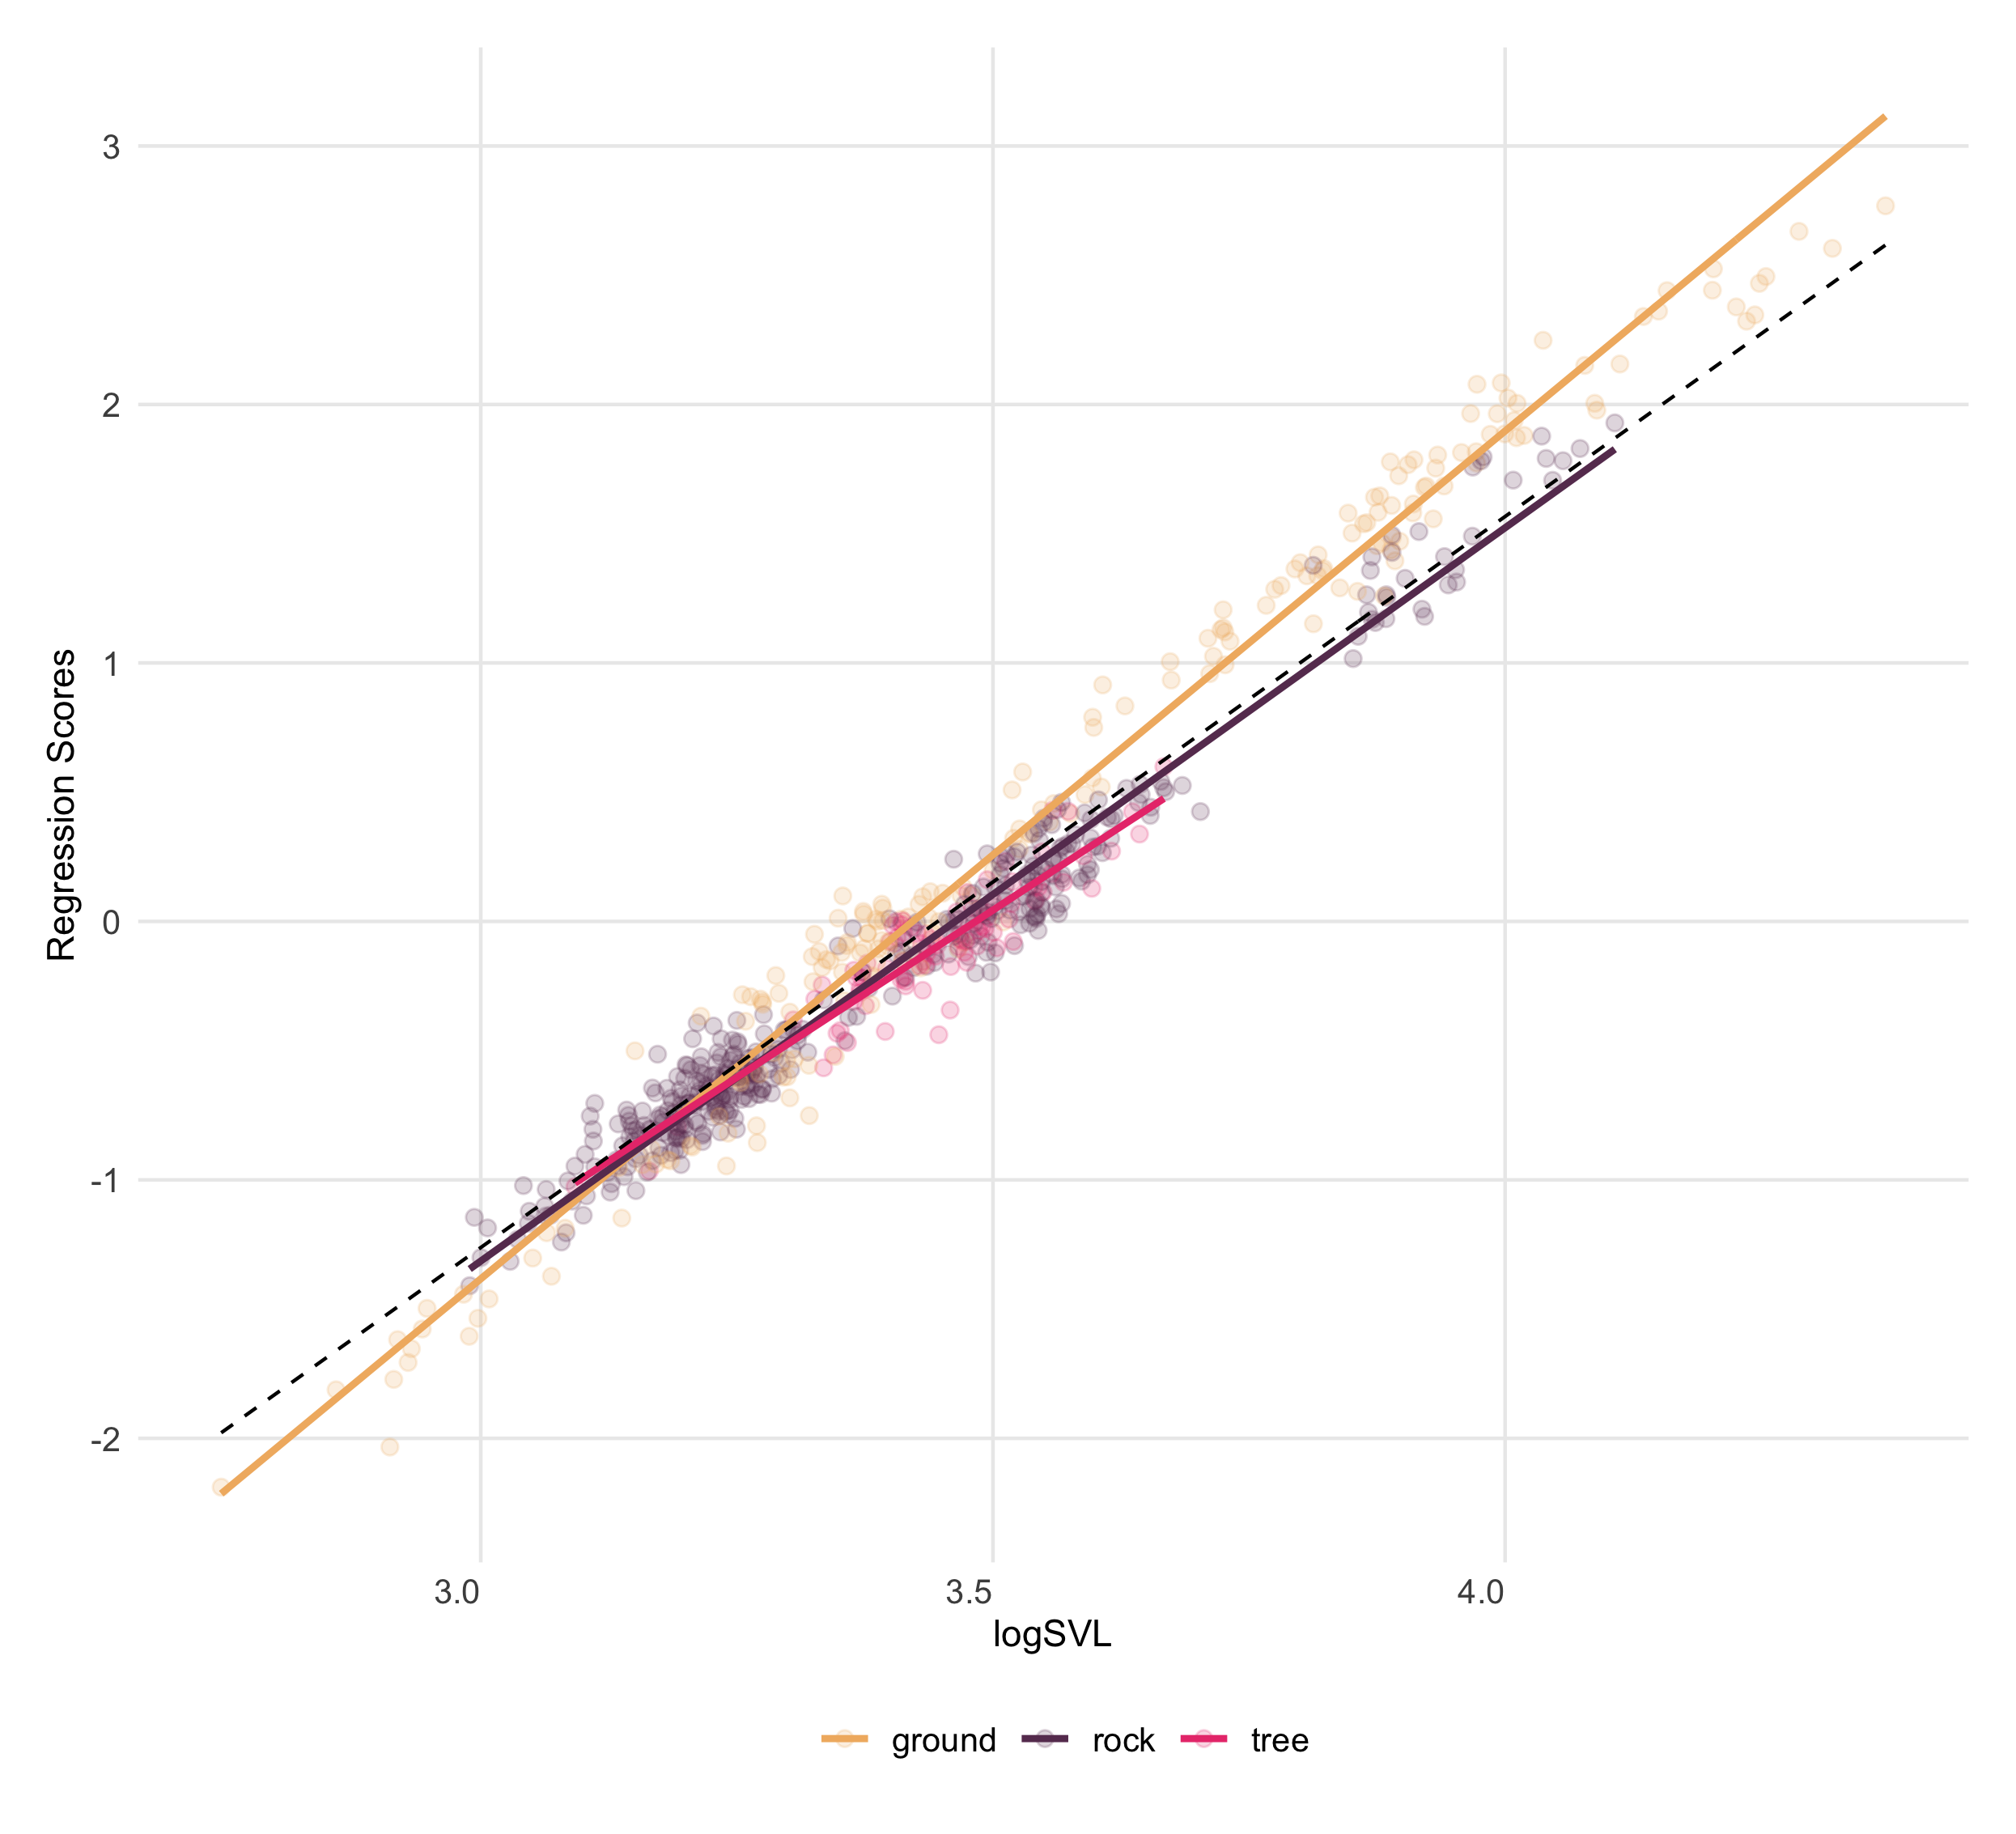
\includegraphics[width=1\linewidth]{Figs/figure_2_ggplot} 

}

\caption{Plot of regression scores and predicted lines representing the relationship between linear body measurements and size (SVL). Individuals are colored by habitat use: ground (beige), rock (dark purple), and tree (magenta). Isometric trend represented by the dashed line.}\label{fig:unnamed-chunk-5}
\end{figure}

\newpage

\begin{figure}

{\centering 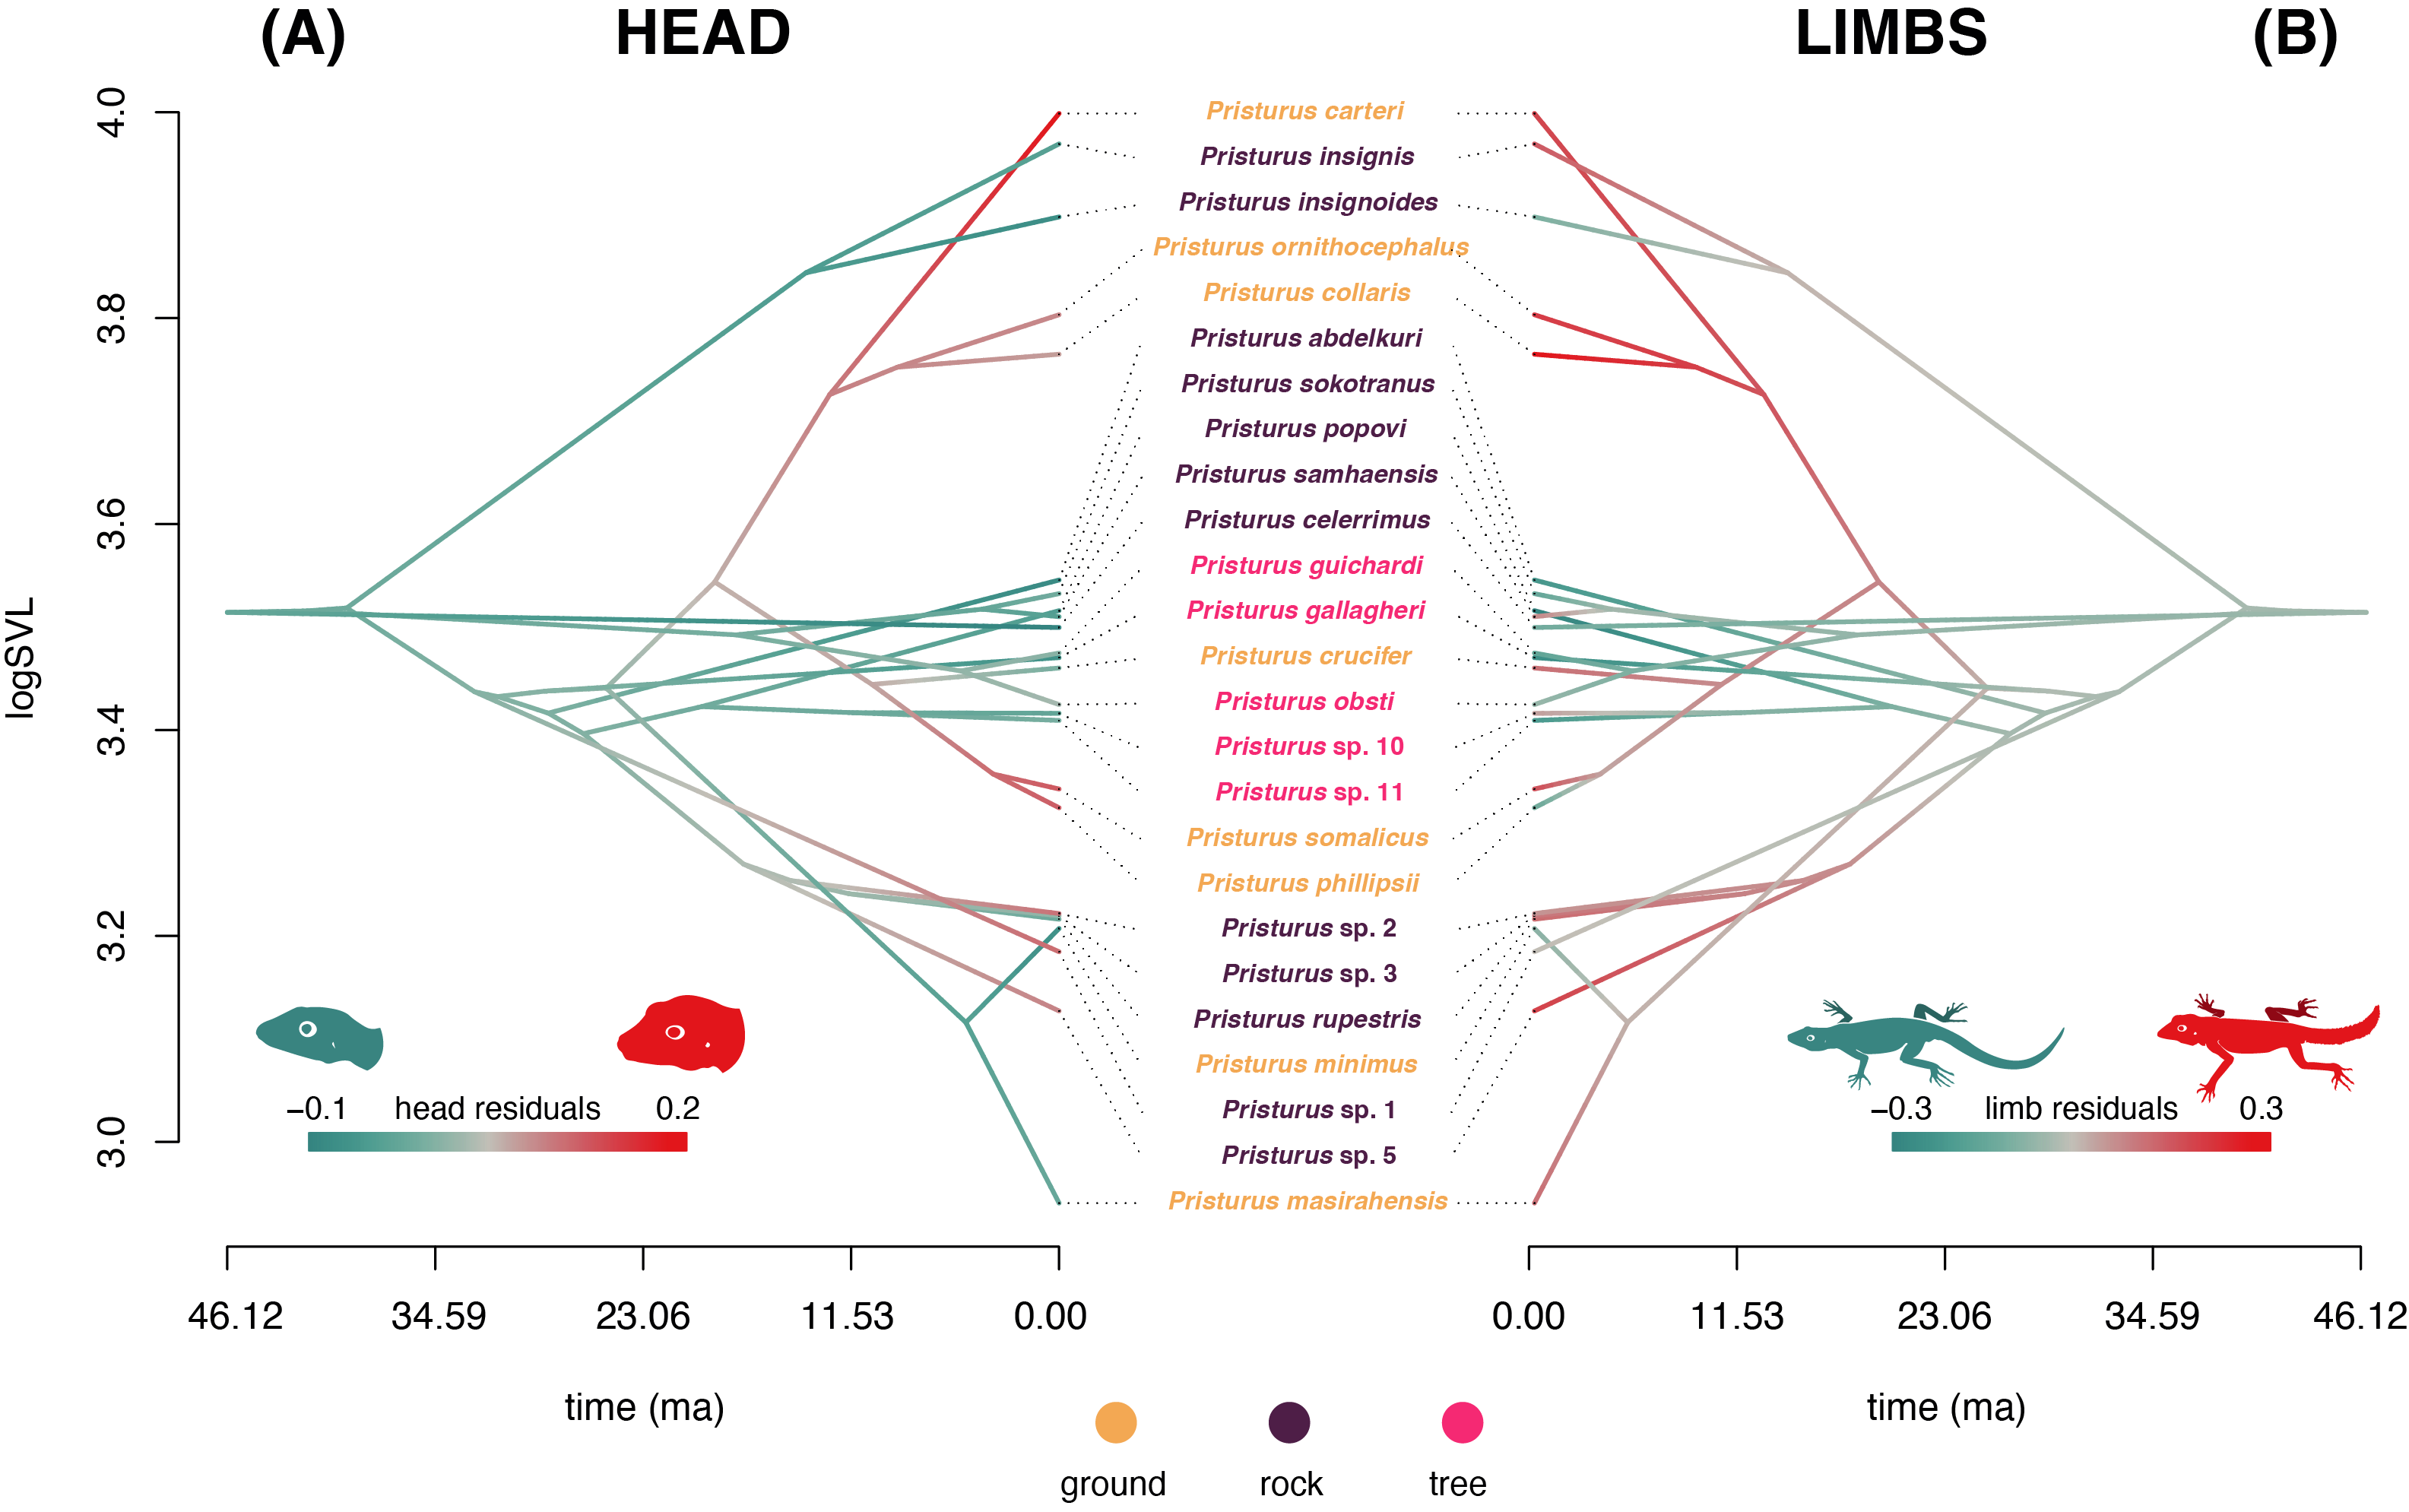
\includegraphics[width=1\linewidth]{Figs/figure_3_Pristurus_allometry_traitgram_legends} 

}

\caption{Traitgrams showing the evolution of body size (SVL) through time based on the phylogenetic tree of \textit{Pristurus}. Colors represent an evolutionary mapping of residuals from phylogenetic regressions describing the relationship of (A) head morphology versus body size, and (B) limb proportions versus body size (see text for descriptions). Species names are colored by habitat use: ground (beige), rock (dark purple), and tree (magenta).}\label{fig:unnamed-chunk-6}
\end{figure}

\newpage

\begin{figure}

{\centering 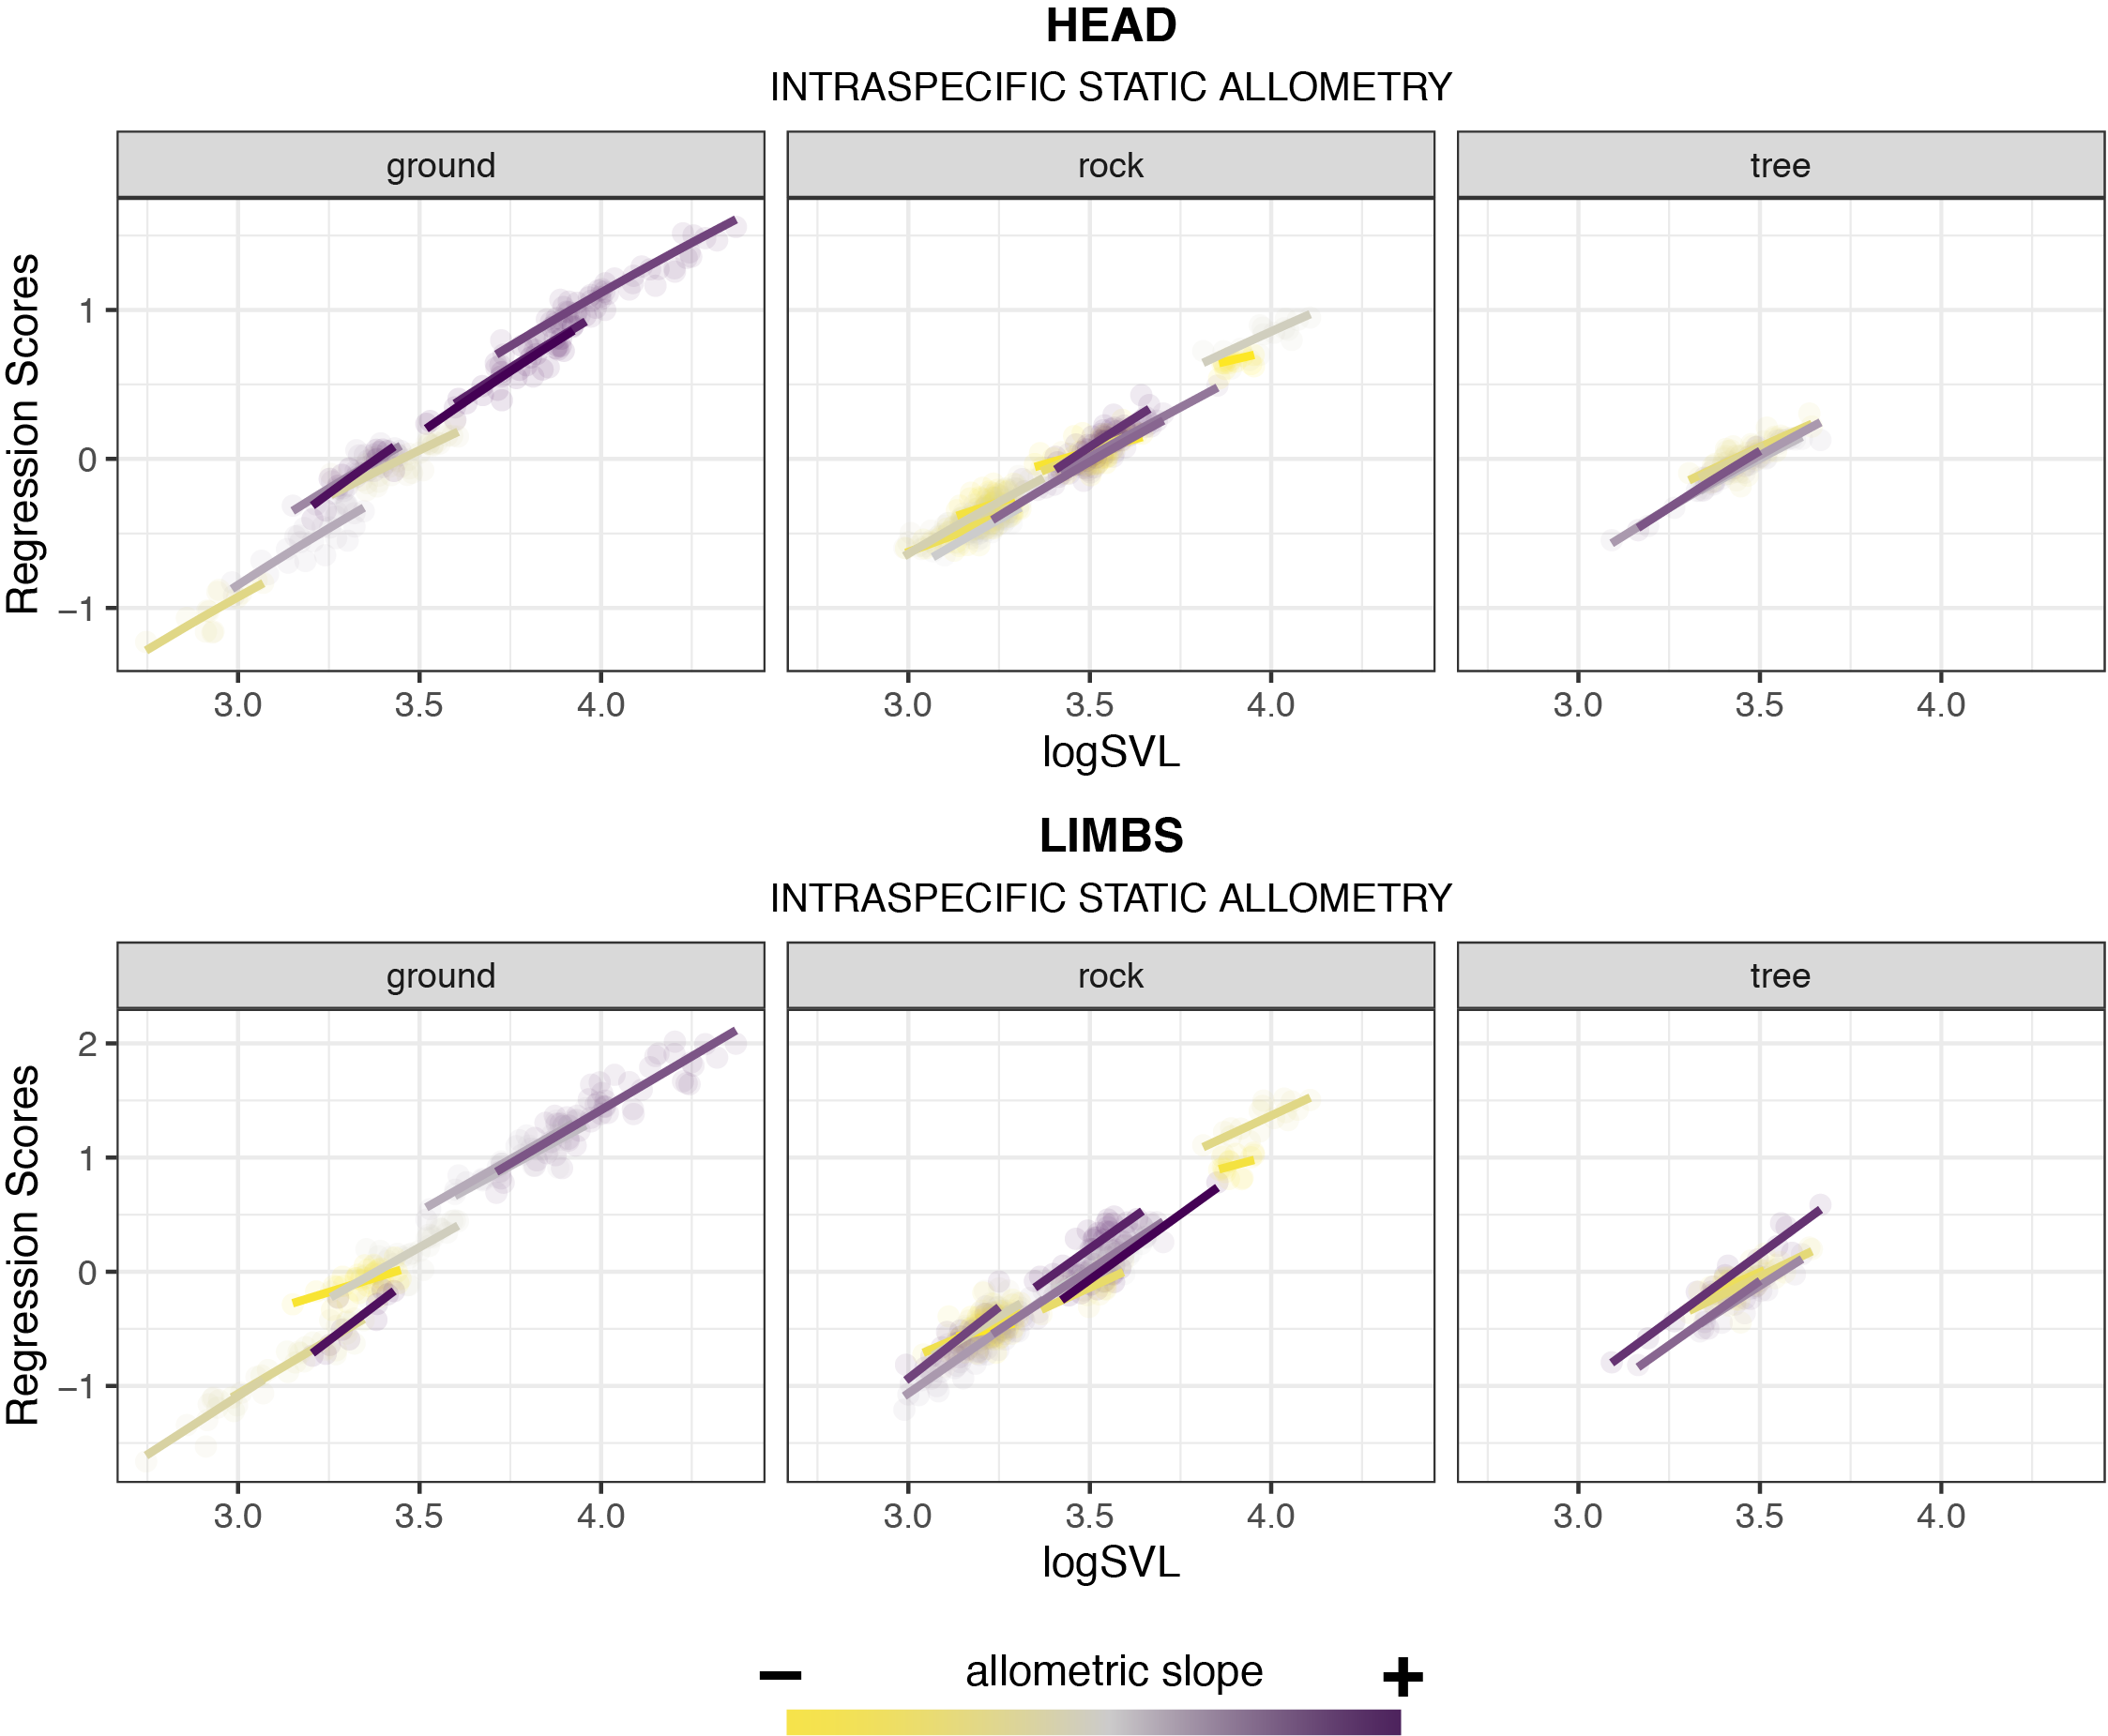
\includegraphics[width=1\linewidth]{Figs/figure_4_static_allometry_v3} 

}

\caption{Patterns of static allometry for each species for head traits (upper panel) and limb traits (lower panel). Species are separated by their habitat groups and colored by the magnitude of their regression slope (purple: steeper slopes, yellow: shallower slopes).}\label{fig:unnamed-chunk-7}
\end{figure}

\newpage

\textbackslash begin\{figure\}

\{\centering 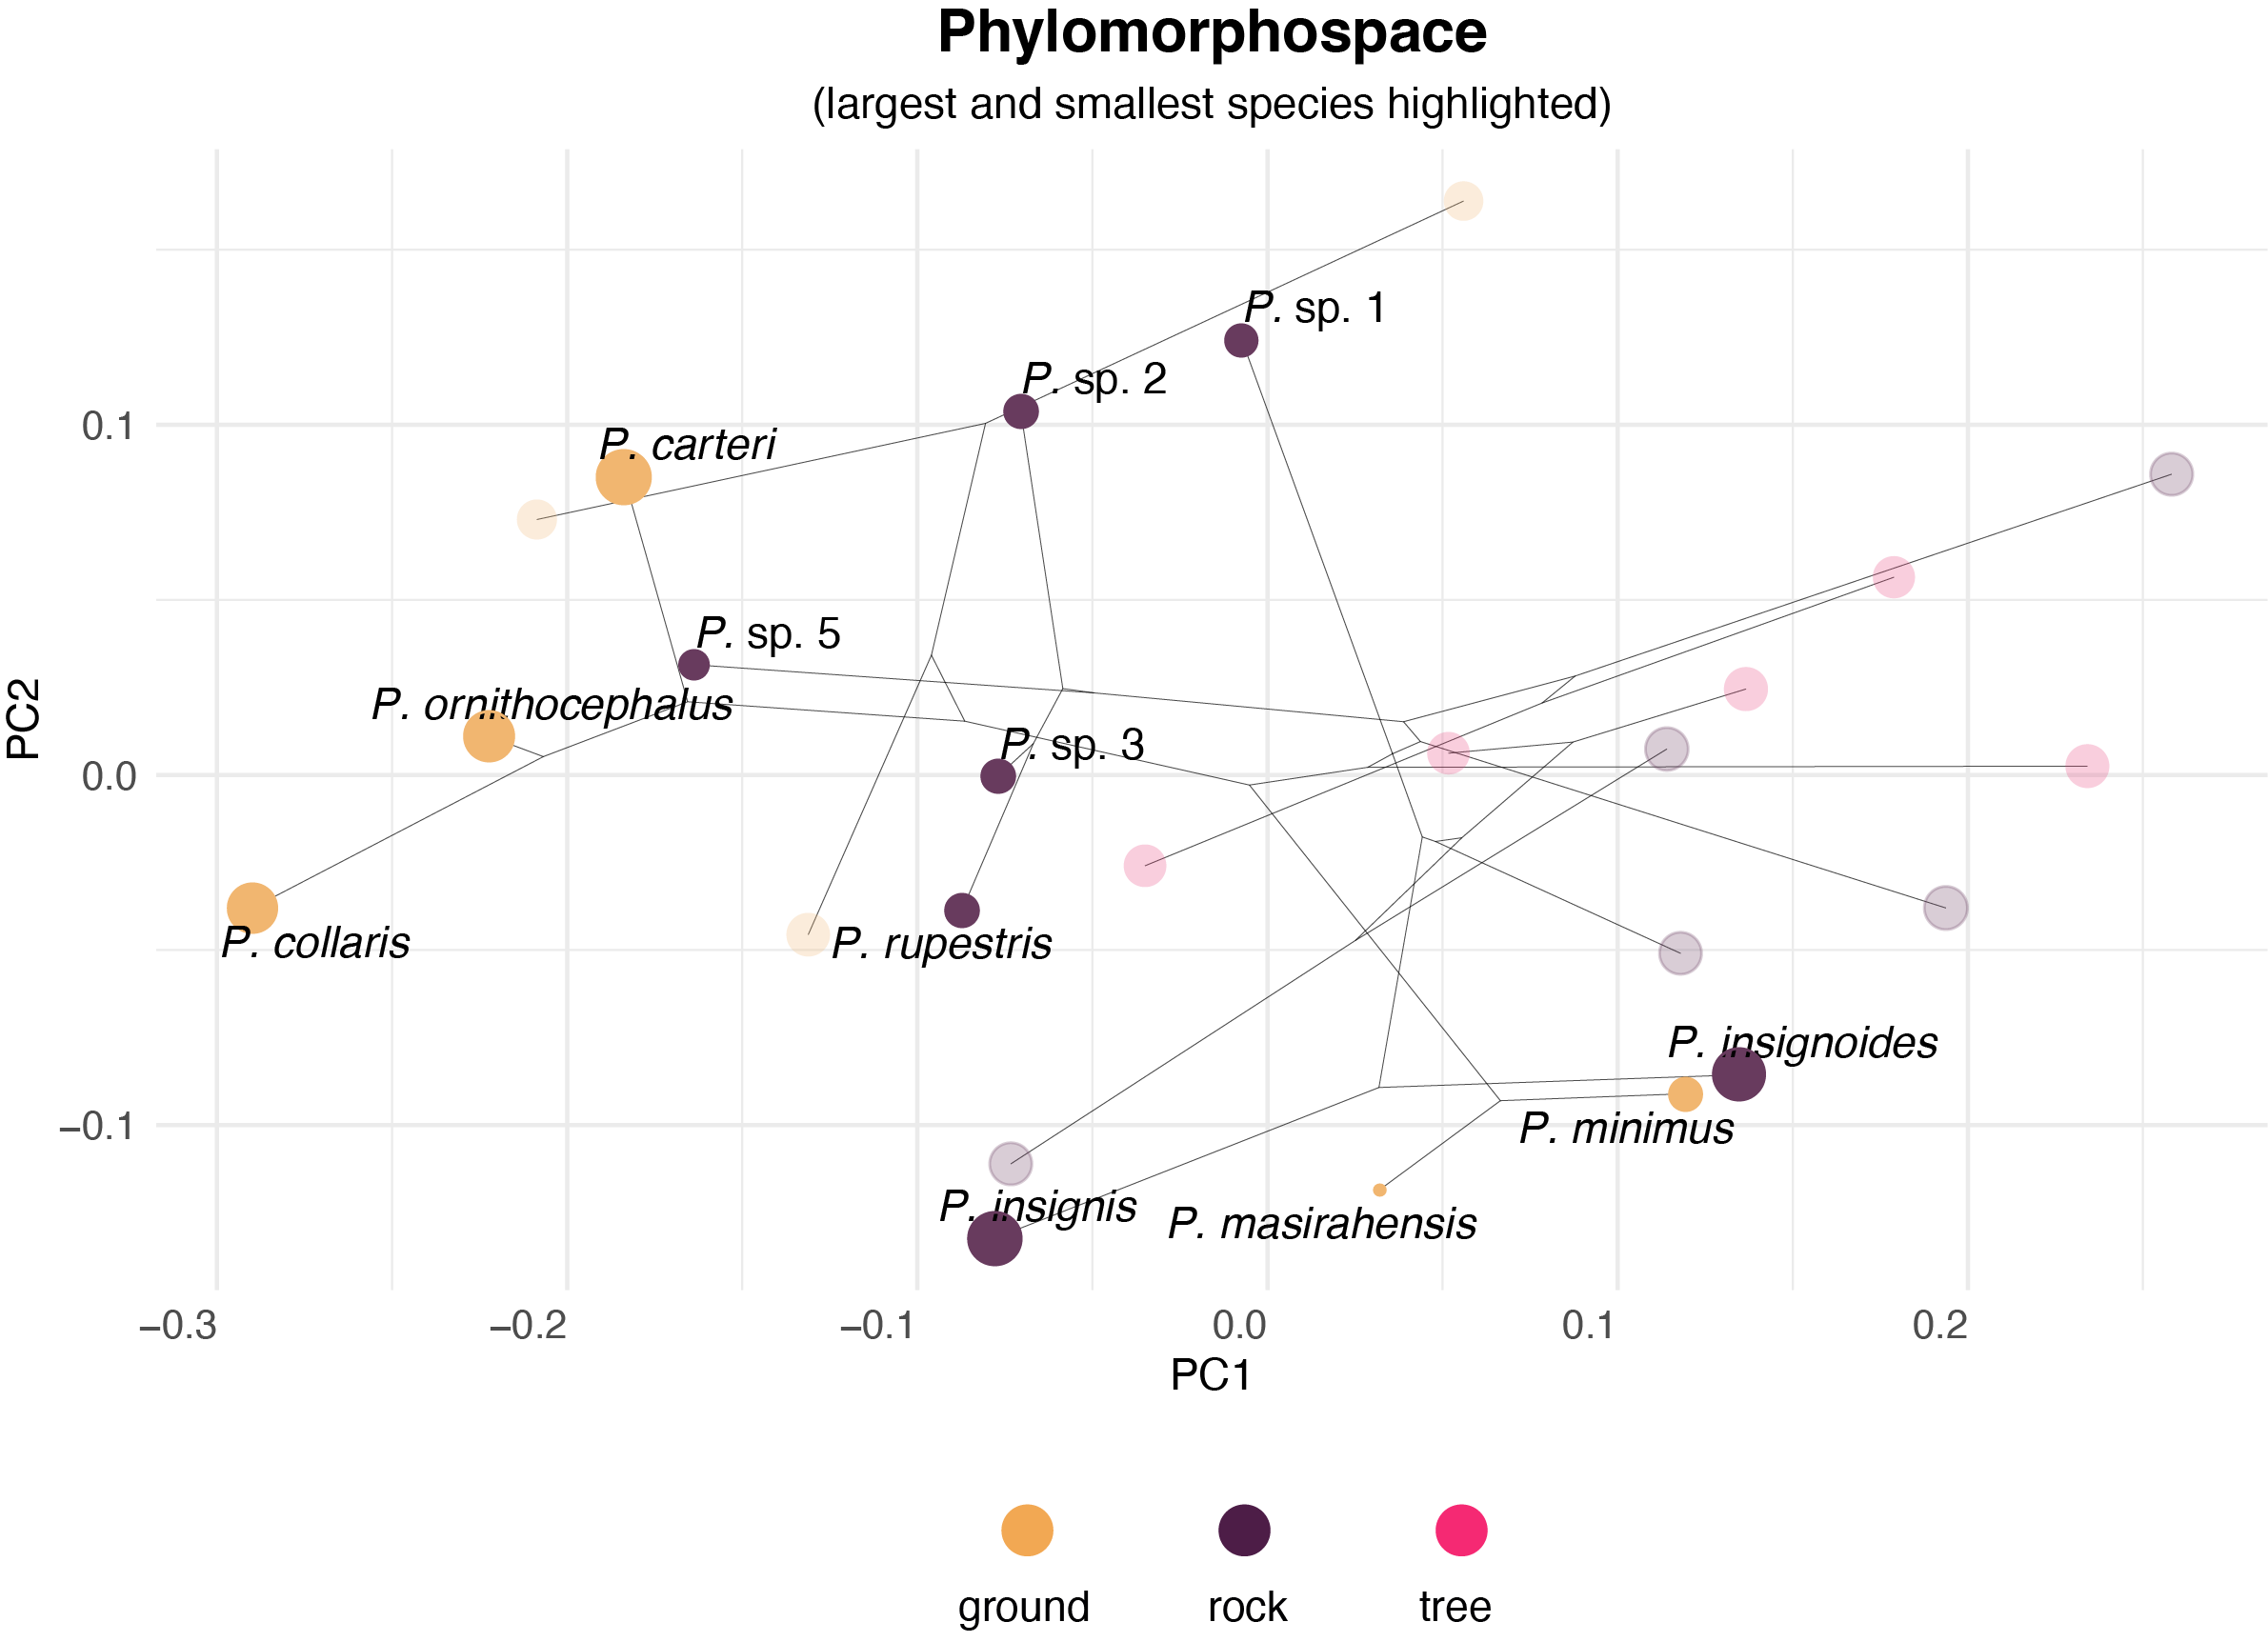
\includegraphics[width=1\linewidth]{Figs/figure_5_phylomorphospace_large_small}

\}

\textbackslash caption\{Phylomorphospace of \textit{Pristurus}, based on
residuals from a phylogenetic regression of body measurements on size
(SVL). Species means are colored by habitat use: ground (beige), rock
(dark purple), and tree (magenta). Large and small rock-dwelling and
ground-dwelling are highlighted with darker colors to highlight their
differentiation and relative positions in morphospace. Point size is
proportional to mean species body size. 79\% of the total variation is
displayed in the first two PC axes (PC1 = 62.8\%; PC2 =
16.3\%).\}\label{fig:unnamed-chunk-8} \textbackslash end\{figure\}

\newpage

\begin{figure}

{\centering \includegraphics[width=1\linewidth]{Figs/figure_6_Pristurus_allometry_rescaledSVL_horizontal} 

}

\caption{Representative specimens (based on real specimens) from large and small \textit{Pristurus} species, colored by habitat use: ground (beige) and rock (dark purple). Specimens are scaled to a common body size (SVL, gray rectangles) to emphasize the relative differences in limb and head proportions. Relatively slender-headed and short-limbed species shown on the left. Original scale shown as the gray bar.}\label{fig:unnamed-chunk-9}
\end{figure}

\end{document}
